\chapter{A Concept for an Exergame for Elderly}
\label{chap:concept}
This chapter is about the second and third activity in the cycle of user centered design, \emph{specifying requirements} and \emph{producing design solutions} (see Figure \ref{userdesign}). Based on findings from workshop 1 and theory presented in earlier chapters, we have created system requirements and designed a concept for an exergame for elderly. The exergame concept, from now on referred to as "the exergame" or the "game", focuses on including movement and exercise in real-life and well-known activities. This will be provided in an entertaining and motivating way. We will present the requirements this exergame is built upon, before we describe the exergame in more detail. This will include games and challenges, goals, obstacles, and how to achieve points. In addition to the exergame, we have also designed a menu. This is based on a course in human-computer interaction (HCI) at NTNU and guidelines for developing interfaces for elderly. 

The exergame presented, is based on theory of how to design video games, as discussed in Chapter \ref{chap:vg}, and can serve as a part of a design document, according to what is described in Section \ref{sec:designphase}. We acknowledge that not all the elements that should be included in a design document are present in this chapter.

When creating the exergame, our prime focus has been on the intended user group. The game is based upon the requirement specification, presented in Section \ref{sec:req}. In addition to this, the informants' feedback are emphasised. The figures in this chapter are prototypes which present scenarios from the exergame. These were made with the intention of presenting the idea and design for the exergame for a group of elderly in a second workshop, and the focus has therefore been on making prototypes that give the users a realistic impression of the final result. The details of our choice of prototypes are provided in Section \ref{sec:prototypes}. The prototypes presented in this chapter will be in English, to be in accordance with the language this report is written in. The original prototypes are in Norwegian and can be found in Appendix C and D. The sources for where we found the pictures used as background and as elements in our prototypes, will also be presented here. 

We will start by presenting the system requirements in Section \ref{sec:req}, before we continue with describing our exergame with its story and included elements. Various scenarios will be presented with the use of medium-fidelity prototypes in Section \ref{sec:outinthenature}. Functional design, presented in Section \ref{sec:functionaldesign}, will give a concrete representation of one possible level of each of the proposed games. Design and description of the menu for the exergame are presented in Section \ref{sec:menu}. This chapter can serve as a part of a design document that can be used by developers to understand and design this exergame.  

\section{Requirements}
\label{sec:req}
We have created a list of requirements for the exergame, which specifies what the system shall do, and which constraints the system shall hold. The requirements have been developed with foundation in all theory presented in the earlier chapters, as well as findings from workshop 1. We have written requirements according to the definition of requirement specification, presented in Section \ref{sec:fourpillarsofdesign}, and they are therefore divided into functional and non-functional requirements. In the exergame we have mostly focused on the functional requirements, and interface requirements, which is a subsection of non-functional requirements. 

We will support our requirement specification by referring to relevant references, findings from workshop 1 (referred to as fw1), motivational factors from Section \ref{subsec:motivator} (referred to as m.x), and guidelines listed in Section \ref{sec:summaryguidelines} and \ref{subsec:golden} (referred to as g.x or e.x respectively). In addition, we will draw references to the GameFlow model \cite{sweetser} (referred to as gf), which holds important elements included in our exergame. These will be listed in the rightmost column. It is important to acknowledge that the requirements also are based upon our own ideas, thoughts and opinions. 

\subsection{Functional Requirements}
The functional requirements in Tables \ref{tab:func1}, \ref{tab:func2} and \ref{tab:func3} present the services and functionality the exergame shall offer.

\begin{minipage}{12 cm}
\begin{table} [H]
\centering
\begin{tabular}{|>{\raggedright}p{0,7cm}|p{8,6cm}|p{1,7cm}|}
\hline
\textbf{No.} & \textbf{Requirement} &  \textbf{Ref.}\\ \hline
1.1 & The system shall be an exergame that emphasises exercise and physical movement. & \cite{project} \\ \hline
1.2 & The system shall have a fun and entertaining story with focus on game play.  & \cite{project} \cite{zyda2005visual} \\ \hline
1.3 & Exercise shall be subordinate to the story. & \cite{zyda2005visual} \\ \hline
1.4 & The system shall meet the diversity in people. & \cite{project}, g.1, g.10, e.2, m.11, fw1 \\ \hline
1.5 & The system shall provide natural and familiar surroundings and elements. & g.11, fw1\\ \hline
1.6 & The system shall provide natural and familiar activities, challenges, and exercises. & g.11, fw1 \\ \hline
1.7 & The system shall provide both physical and cognitive challenges. & m.8, fw1 \\ \hline
1.8 & The system shall allow for decision making before and during the game. & \cite{understandingvg}, m.9 \\ \hline
1.9 & The system shall provide players with clear instructions on how to use and interact with the game. & g.6, e.8, fw1 \\ \hline
1.10 & The system shall provide players with clear instructions on how to perform various activities, challenges, and exercises. & \cite{project}, g.6, g.8, e.8, m.2, gf, fw1\\ \hline
1.11 & Instructions shall include information about the health benefits gained from playing. & m.3, fw1\\ \hline
1.12 & Instructions shall be given during game play when appropriate. This shall be done to avoid the need to memorise information. & g.6, g.9, e.8, gf \\ \hline
    \end{tabular}
    \caption[Functional requirements, part 1]{Functional requirements \footnote{g - guidelines, e - guidelines from the Eight Golden Rules, m - motivators, gf - elements from the GameFlow model, fw1 - findings from workshop 1}}
    \label{tab:func1}
\end{table} 
\end{minipage}

\begin{minipage}{12 cm}
\begin{table} [H]
\centering
\begin{tabular}{|>{\raggedright}p{0,7cm}|p{8,6cm}|p{1,7cm}|}
\hline
\textbf{No.} & \textbf{Requirement} & \textbf{Ref.} \\ \hline
1.13 & The system shall give players the time they need to read instructions. & g.46, m.9, fw1 \\ \hline 
1.14 & The system shall allow players to skip instructions. & e.7, m.9, gf, fw1 \\ \hline 
1.15 & Players shall be given feedback on their actions. &  e.3, gf, fw1 \\ \hline
1.16 & Feedback given shall be positive and motivating. & \cite{project}, g.7, gf \\ \hline
1.17 & Feedback shall only be given when appropriate. Interruptive feedback shall be avoided during game play. & g.9, gf, fw1 \\ \hline
1.18 & The system shall be a progression game. & \cite{understandingvg}, g.17, gf \\ \hline
1.19 & The system shall have small subtasks with clear goals. & g.17, m.6, gf, fw1\\ \hline
1.20 & Players shall be informed about progression and results. & g.18, e.3, m.7, gf, fw1 \\ \hline
1.21 & The system shall allow multi-play. & g.12, m.9-11, fw1 \\ \hline
1.22 & Multi-play shall have the possibility to be performed both as collaboration and competition. & gf, fw1\\ \hline
1.23 & Players shall be given the possibility to choose preferred difficulty level. & g.17, g.19, m.9, m.11, gf, fw1\\ \hline
1.24 & The system shall allow for players to choose individual difficult levels. & g.19, m.9, m.11, gf, fw1\\ \hline
1.25 & The system shall be able to adjust difficulty level after players' progression. & gf, fw1 \\ \hline
    \end{tabular}
    \caption[Functional requirements, part 2]{Functional requirements \footnote{g - guidelines, e - guidelines from the Eight Golden Rules, m - motivators, gf - elements from the GameFlow model, fw1 - findings from workshop 1}}
    \label{tab:func2}
\end{table} 
\end{minipage}

\begin{minipage}{12 cm}
\begin{table} [H]
\centering
\begin{tabular}{|>{\raggedright}p{0,7cm}|p{8,6cm}|p{1,7cm}|}
\hline
\textbf{No.} & \textbf{Requirement} & \textbf{Ref.} \\ \hline
1.26 & Activities provided by the system shall include exercises for all muscle groups. & \cite{aktivitetsbok} \\ \hline
1.27 & Exercises used shall be proved to be good for training for elderly. & \cite{project}, g.21 \\ \hline
1.28 & Activities shall be possible to perform both sitting and standing. & g.20, m.9, m.11 \\ \hline
1.29 & The system shall give the players the possibility to choose gender on their character. &  g.10, g.14, m.9, m.11 \\ \hline
1.30 & The system shall always provide players with the possibility to reverse their actions. & g.48, e.6, m.9 \\ \hline
1.31 & The system shall create a user profile where players' progression and results can be saved. & \cite{project}, g.23 \\ \hline
1.32 & The system shall provide players the possibility to share their profile, or part of their profile, with friends. &  gf \\ \hline
1.33 & The system shall be able to be used as a tool for physiotherapists. & \cite{project}, g.22 \\ \hline
1.34 & The system shall give physiotherapists the possibility to set parameters to customise the exergame for each individual patient. & \cite{project}, g.1, g.39  \\ \hline
1.35 & The system shall give physiotherapists access to players'/patients' profiles. & \cite{project}, g.23\\ \hline  
\end{tabular}
\caption[Functional requirements, part 3]{Functional requirements \footnote{g - guidelines, e - guidelines from the Eight Golden Rules, m - motivators, gf - elements from the GameFlow model, fw1 - findings from workshop 1}}
\label{tab:func3}
\end{table} 
\end{minipage}

These requirements will be used as a foundation for the exergame, and they will serve as input to the functional design presented in Section \ref{sec:functionaldesign}. Requirement 1.33 - 35 focus on the physiotherapists' view of the system. As previously mentioned, we have in this thesis emphasised interface design for the end users which are elderly people. However, it is important that these three requirements are included in future work on the exergame. This is because we in our previous project \cite{project} evaluated physiotherapists to be the proper customer for the game. We believe that in today's market the game will not experience success going straight to the end users \cite{project}.  

\subsection{Non-Functional Requirements}
The non-functional requirements presented in Tables \ref{tab:nfunc1} and \ref{tab:nonfunc2} describe constraints to follow for the exergame to ensure good usability in terms of interface design.

\begin{minipage}{12 cm}
\begin{table} [H]
\centering
\begin{tabular}{|>{\raggedright}p{0,7cm}|p{8,4cm}|p{1,9cm}|} 
\hline
\textbf{No.} & \textbf{Requirement} & \textbf{Ref.} \\ \hline
2.1 & The system shall provide good graphics in 3D, which makes the game world look real. & \cite{understandingvg}, g.15 \\ \hline
2.2 & The system shall use characters to portray the players. & \cite{understandingvg}, g.15 \\ \hline
2.3 & The system shall provide sound and music appropriate for the user group. & g.10, m.13, fw1 \\ \hline
2.4 & The system shall provide sound and music appropriate for the game theme and the intensity in the current activity. & \cite{umlapproach}, m.13, fw1 \\ \hline
2.5 & The system shall have a menu, which is used by players to make choices about game play. & g.5\\ \hline
2.6 & The menu shall be clear, simple, and intuitive. & g.4, g.31, e.8, gf, fw1 \\ \hline
2.7 & The menu shall be consistent. & g.32, e.1 \\ \hline
2.8 & Menu buttons shall not be too sensitive. & fw1 \\ \hline
2.9 & Menu buttons require "push" to perform any action. & fw1\\ \hline
2.10 & The navigator shall not be too sensitive. & fw1\\ \hline
2.11 & The navigator shall be clear. & fw1\\ \hline
2.12 & Information shall be easy to see, and understand. & g.47, e.8\\ \hline
2.13 & Information shall be written in a familiar language with everyday words. & g.30\\ \hline
\end{tabular}
\caption[Non-functional requirements, part 1]{Non-functional requirements, interface requirements \footnote{g - guidelines, e - guidelines from the Eight Golden Rules, m - motivators, gf - elements from the GameFlow model, fw1 - findings from workshop 1}}
\label{tab:nfunc1}
\end{table} 
\end{minipage}

\begin{minipage}{12 cm}
\begin{table} [H]
\centering
\begin{tabular}{|>{\raggedright}p{0,7cm}|p{8,4cm}|p{1,9cm}|} 
\hline
2.14 & Information shall be written with an easy-to-read font in an appropriate size. &  g.2, g.24-28\\ \hline
2.15 & There shall be clear contrast between background colour and text colour. & g.37-43 \\ \hline
2.16 & Elements that are essential to the game shall stand out. & g.31, g.43\\ \hline
2.17 & The system shall avoid using elements that are unnecessary for current situation.  & gf, fw1\\ \hline
\end{tabular}
\caption[Non-functional requirements, part 2]{Non-functional requirements, interface requirements \footnote{g - guidelines, e - guidelines from the Eight Golden Rules, m - motivators, gf - elements from the GameFlow model, fw1 - findings from workshop 1}}
\label{tab:nonfunc2}
\end{table} 
\end{minipage}

\section{The Overall Story Line}
\label{sec:outinthenature}
We will now present the story line of the exergame. This will be based on the requirements provided in the tables above. We will refer to the relevant requirement with [req. no] throughout the presentation. 

"Out in the Nature" ("Ut i naturen" in Norwegian) is the title of our exergame. This is a game based on a forest theme and it consists of real-life activities that are familiar to most people [req. 1.5]. The different activities are natural to find and do in the forest or in the nature, hence the game name. The goal is to experience beautiful nature while playing, and at the same time exercise and achieve physical activity [req. 1.3-4]. Bringing the beautiful nature "to life" is achieved by presenting the game with 3-dimensional graphics [req. 2.1]. The exergame consists of five individual games, one longer, compounded game that will engage the whole body, and four, shorter single games with various challenges and exercises, both for the mind and body [req. 1.7, 1.26].        

We have used familiar elements that can be found in the forest, i.e. rocks, creeks, and logs. When we have chosen to use other elements, these are well-known, and easy to relate to for elderly people [req. 1.5]. One example is hearts and their relation to health. In addition, our intention has been to avoid unnecessary details that can lead to confusion and distraction [req. 2.17], in accordance with simplistic design, discussed in Section \ref{sec:simplicity}. Music and sound effects in the game will be natural when possible [req. 2.4], like birds twittering and the wind in the trees. The informants mentioned that classical music, e.g. Mozart, would be more suitable than the computer-made pop music that was used in the commercial games we presented for them. An idea is therefore to use classical music that will fit a walk in the beautiful nature a warm summer day [req. 2.3]. When there are challenges and activities that require intensity, the idea is to use music with a rhythm, without being noisy [req. 2.4]. We will not present any specific music examples suitable for this exergame, since that is outside our area of competence. 

The player will be presented in the game as a character with "real-life" features [req. 2.2]. As described in Section \ref{subsub:fictionalworld}, the player character can be described by three different categories: avatars, actors and roleplaying. From the definition, the player character here will be an actor. However, in commercial Kinect games the player character is called an avatar, and we will therefore do the same. They do not have a distinct personality except from being "a normal human being", but they are well integrated into the story. We will use two different male and female avatars [req. 1.3, 1.29], to meet with the requirement of having two simultaneously players [req. 1.21]. All characters are dressed in training outfits; females in training leggings and t-shirt, and males in long pants and t-shirt. The different characters will have different colours on their t-shirts to make it easy for the players to distinguish between them. The male avatars have either blue or green t-shirts, while the female avatars have either yellow or pink t-shirts. The males have short hair, and the females have half-long hair. For convenience, the characters will have international names, like Anne, Eva, Charles and David. The avatars will be seen in a third-person perspective. This is because it is important for the player to see the avatar of herself to see if she is doing the exercises correctly. 

"Out in the Nature" is meant to be an exergame for elderly, but it is important to not just focus on the exercise. This exergame has an entertaining and motivating story, which is the main focus in the game. The exercises are only subordinate to the story [req. 1.1-3]. However, we will include the opportunity for the player to choose which part of their body they want to exercise. In the first step in the menu, the player is given the choice of how she wants to play, see Figure \ref{fig:menuStart}. The player can choose to play the compounded game, choose to play based on exercising a preferred muscle group, or the player can choose among the four single games [req. 1.8]. Our choice of including this in the exergame is based upon feedback from workshop 1, where the informants stated that it was important to make own decisions on how, and when, they would like to work out.                     

\begin{figure} [H]
\centering
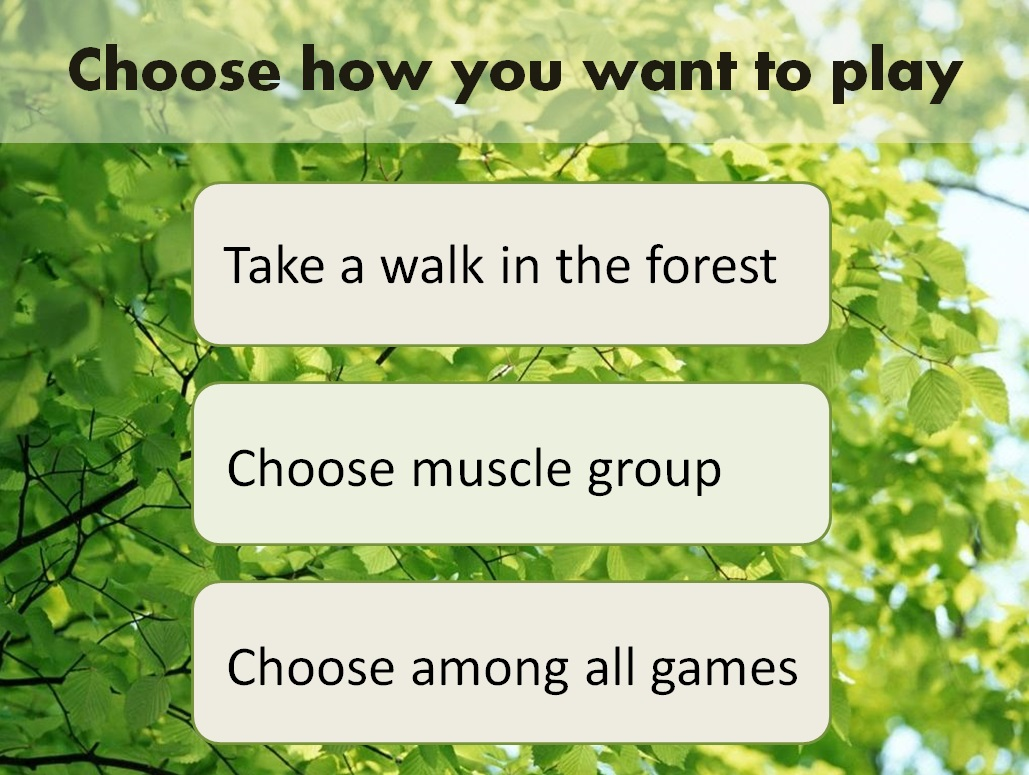
\includegraphics[scale=0.24]{choosePlay.jpg}
\caption[The menu - start]{In the first menu step, the player is given the opportunity to choose how they would like to play. The can go for the compounded game, play according to a chosen muscle group, or they can choose among the four single games.}
\label{fig:menuStart}
\end{figure} 

\subsection{Exercises}
The activities we have selected for the exergame are based upon findings from workshop 1, and our own ideas. However, the main reason for using these activities is because they involve exercises that have been proved to be good for elderly [req. 1.27]. In Section \ref{sec:summaryguidelines}, stepping, balance and strengthening exercises are proposed as suitable for elderly. These were also suggested as appropriate exercises by The Norwegian Directorate of Health \cite{aktivitetsbok}. In addition, we have used \emph{Øvelsesbanken} \cite{eldretrening}, which is presented in Section \ref{sec:exercisebehaviour}, as a guide to find exercises to use in the exergame. We have picked out 18 exercises from \emph{Øvelsesbanken} that we argue are a good foundation for the exergame. Some exercises chosen are "picking apples" (see Figure \ref{pickingapples}), "walking", and "rowing". All the chosen exercises are presented in Appendix B. Most of the exercises have the possibility to be performed both sitting and standing, to make the exergame available for those who are not able to stand or walk. We got copyright clearance from "Øvelsesbanken" to use their exercises.  

In workshop 1 it was mentioned that the whole range of exercising, from warm-up to stretching, should be included. We have not looked any further into this, as this should be up to professionals, like physiotherapists, to decide. However, it should be easy to implement these requirements in this exergame.


\begin{figure} [H]
\centering
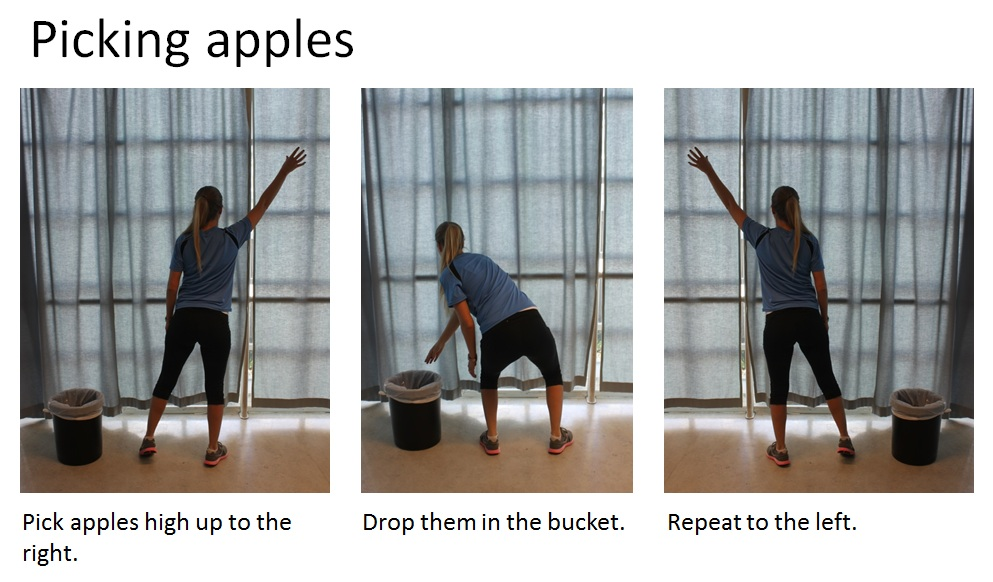
\includegraphics[scale=0.5]{PickingApplesAlone.jpg}
\caption[Exercise - picking apples]{The "Picking apples" exercise from \emph{Øvelsesbanken}.}
\label{pickingapples}
\end{figure}

\subsection{Instruction and Feedback}
In this exergame, the player will be given instruction about the technology, how to play, and how to perform various activities and exercises [req. 1.9-10]. When first starting the exergame, the player will be informed on how to interact with the Kinect sensor and the game. The player will be told that she has to use her body to engage game play, that she has to use her hand to navigate through the menu, and that she can make a choice by "pressing a button". 

In each of the five games there will be instructions informing about the goal of the game, the purpose of the various elements, and how the player should move to perform the activities in the game [req. 1.10]. There will also be provided information of the health benefits gained from performing the various activities [req. 1.11]. When the game starts, the overall purpose and goal are explained. This is for the player to know what is expected from her [req. 1.9-11]. Specific information about the various challenges will not be given all at once, as this will require a lot of memorisation. Therefore, these types of instructions will be given during game play, when there occur situations that makes it appropriate to provide the player with new information [req. 1.12]. This will be when the player meets new elements, obstacles or challenges. Every instruction comes with a button that the player has to push to continue playing. In this way the player is in the control of the game, and can decide for herself when she is finished reading the instruction [req. 1.13]. Figure \ref{fig:kineintro} shows an example of an instruction. The player will always be given the possibility to skip the instructions, so experienced players do not have to watch the same instructions each time she plays [req. 1.14].

During game play, the player will be given appropriate feedback on her actions [req. 1.15-16]. This will be given when she has completed a particular task or activity, to not interrupt the player from performing ongoing tasks [req. 1.17]. Examples will be motivating comments, such as "Congratulations, you did a great job", when the player has accomplished balancing over a log, or "Lift your legs higher to walk faster". While playing, feedback should be given orally by a calm lady voice [req. 2.3]. Textual feedback during game play is avoided to not interfere with immersion and disturb the gaming experience [req. 1.17].  However, text can be chosen instead of voice if it is preferred [req. 1.4]. 

\begin{figure} [H]
\centering

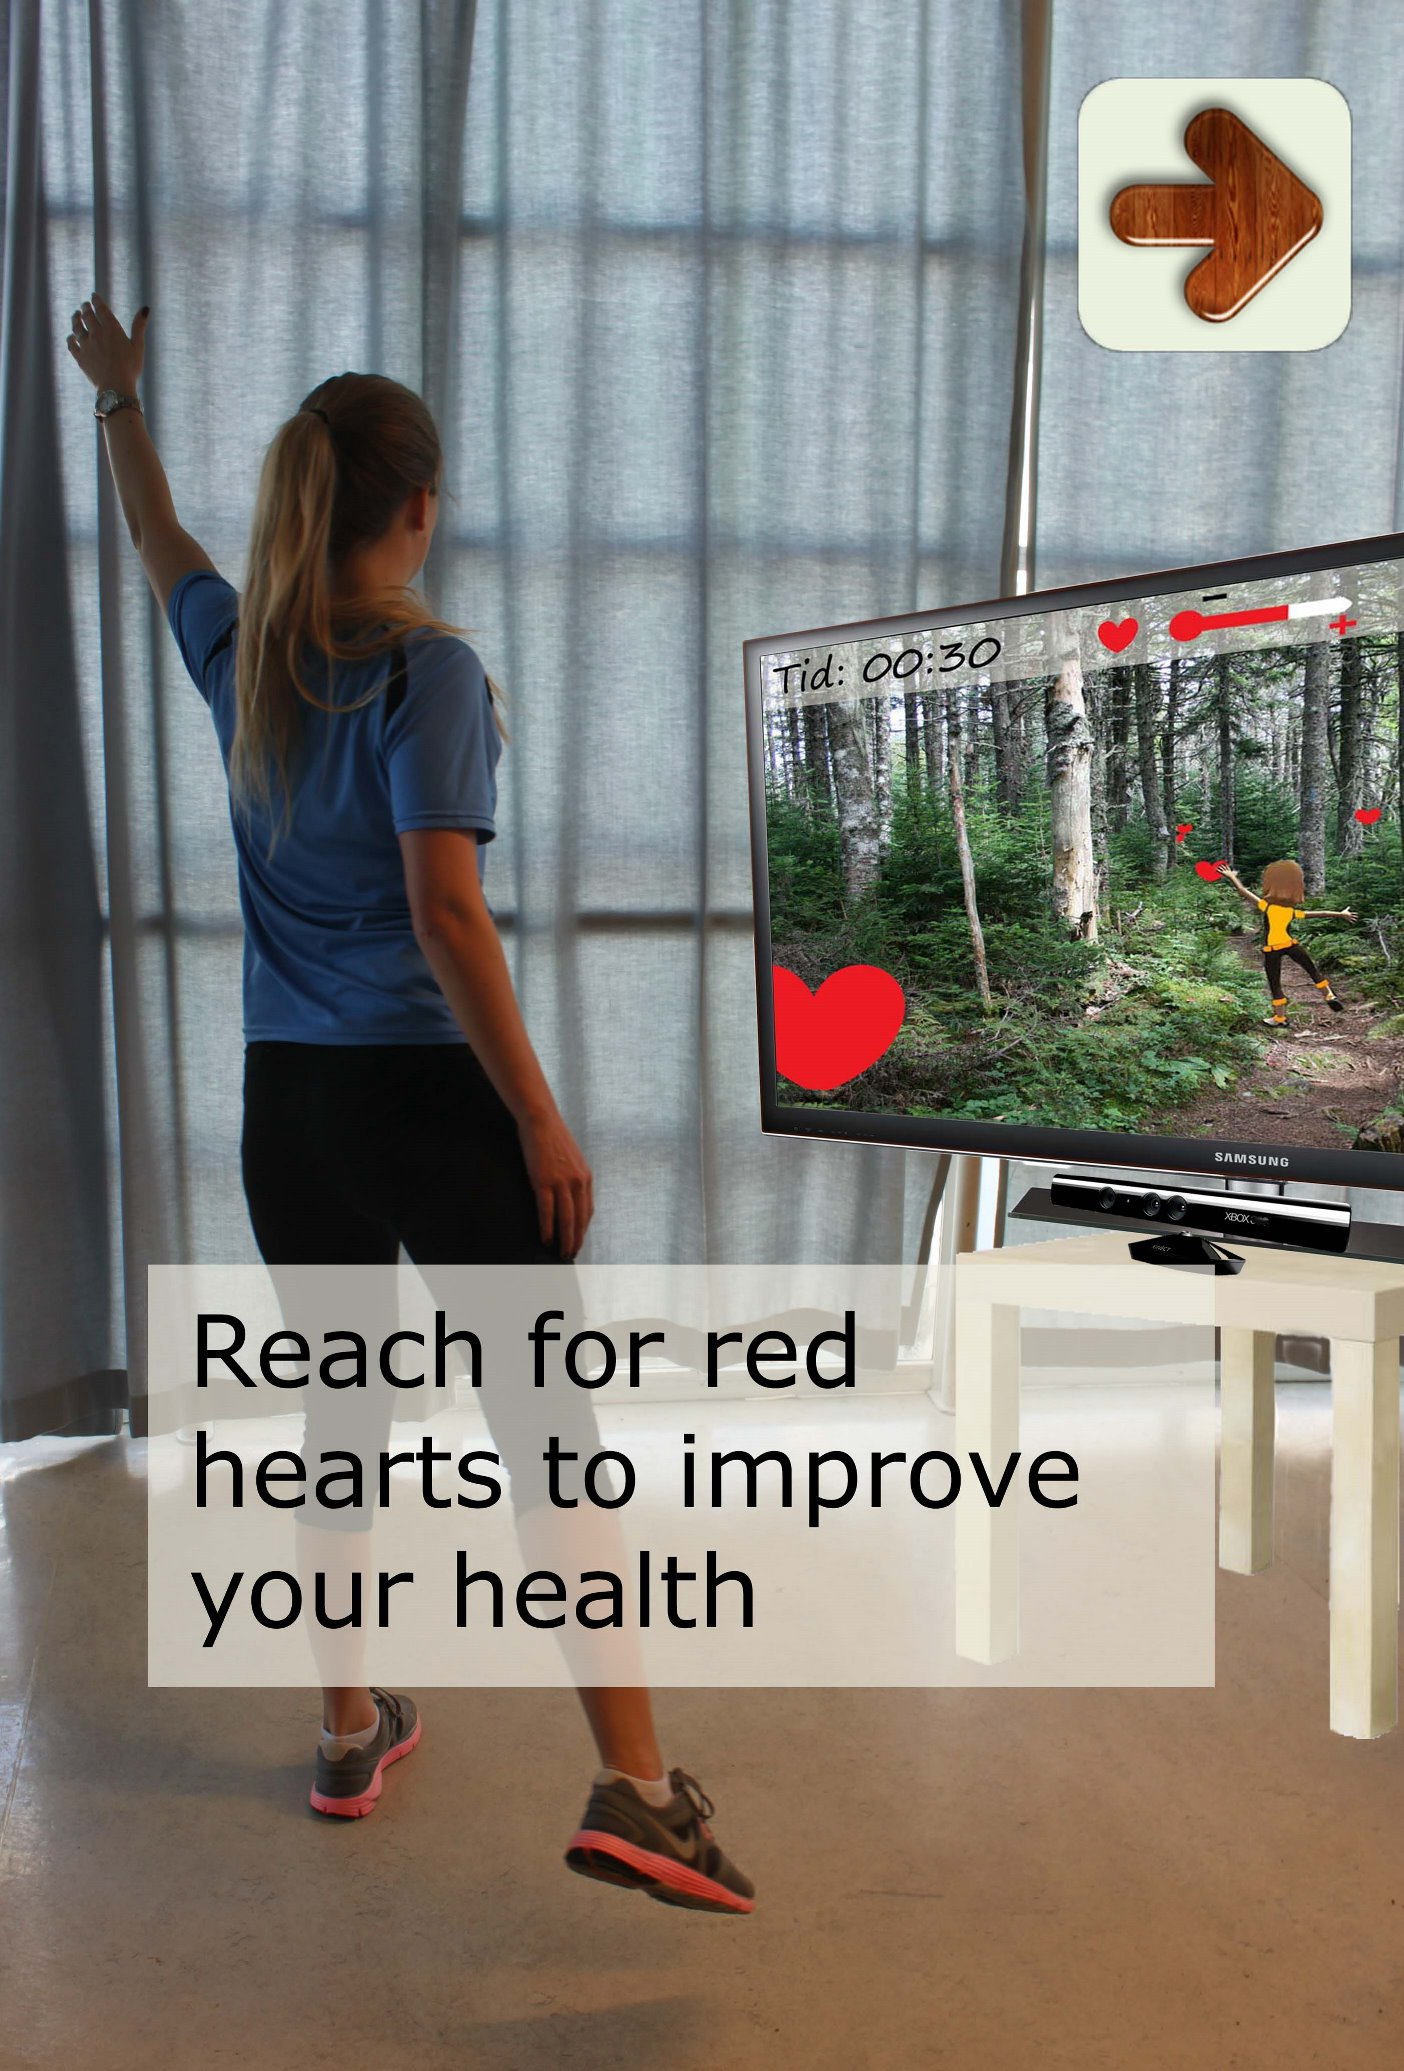
\includegraphics[scale=0.13]{introKineEng.jpg}
\caption[Instruction]{This figure shows an instruction in the exergame. There is a button up in the right corner that will be used to continue with the game when the player is done reading the information.}
\label{fig:kineintro}
\end{figure}

\subsection{Nature Trail}
The main activity in "Out in the Nature" is what we have called "Nature Trail". This involves a walk in the forest with quizzes along the way. The goal for the game is to complete the nature trail as fast as possible, while answering questions, and avoiding obstacles on the way [req. 1.7]. Points will be given according to correct answers on the quiz, which will be shown up in the right corner together with an icon showing a sheet of paper. Because the Kinect sensor can track movements, points will also be given according to how well the player performs the required movements. These points will not be shown as numbers, as movements will be difficult to measure and "grade". Therefore, gain from correct and well-performed movements is shown in a "health-bar" on top of the screen [req. 1.20]. Showing this visually is done to avoid too much detailed information, as suggested by Brox et al. \cite{exergamesforelderly}. A red heart is shown together with the bar to represent health. Points for correct answers on the quiz are separated from points achieved from movements, because the quiz has to do with cognitive skills, while the latter is about physical skills. The time used to complete the nature trail will affect the final result of the "health-bar", as this also reflects how well the player has moved during game play. Figure \ref{fig:hearts} presents a scenario from the exergame, which includes the described elements in the top-bar. "Nature Trail" supports the possibility to choose number of players, as multi-player mode enhances social interaction while playing [req. 1.8, 1.21].  

Progress in the game requires movement, like walking. When walking, the avatar portraying the player will walk into the forest. The bigger movements the player uses, e.g. the higher the player lifts her feet while walking, the higher pace, and "better health" she will achieve. Figure \ref{fig:hearts} shows the avatar in the forest, surrounded by hearts, where the avatar does a wide stretch trying to reach a heart. The hearts will be positioned in a way that will require the player to move to reach for them. Therefore, if the player gathers these hearts, her health will improve due to physical activity [req. 1.3]. Gain from gathering hearts will also be shown in the "health-bar".   

\begin{figure} [H]
\centering
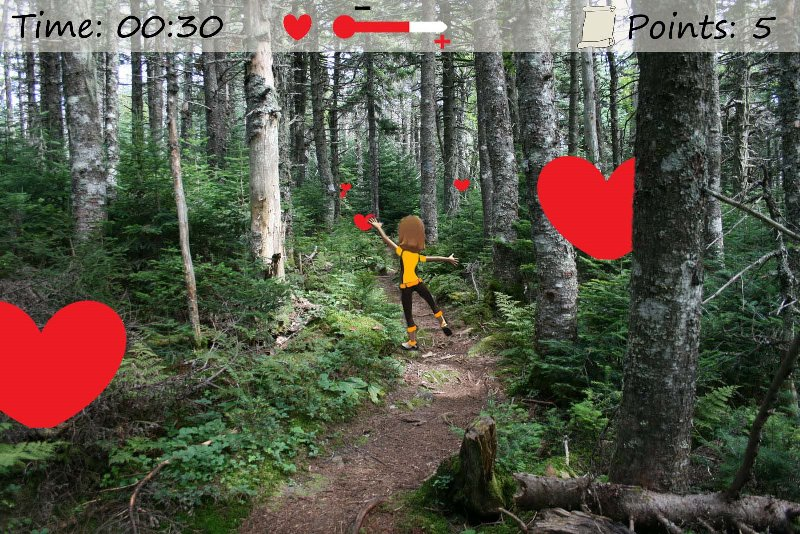
\includegraphics[scale=0.27]{game1engelsk.jpg}
\caption[Nature trail - stretching]{This figure presents a scene from the "Nature Trail" game. We see the avatar in the forest, doing a wide stretch trying to reach a heart. This will result in improved health, shown in the "health-bar".}
\label{fig:hearts}
\end{figure}

The quiz will be shown along the trail as sheets of paper "hanging" on different spots in the forest. The player has to reach for them to get access to the questions. When picking a question, it will pop up and fill the screen (see Figure \ref{fig:quiz}). Four alternatives will be shown, and the player will have to use her hand to navigate to what she believes is the right answer. Questions will be chosen randomly, so the player does not get the same questions each time she plays. The difficulty will also increase in line with number of correct answers [req. 1.25]. The player does not have to answer the quiz to complete the "Nature Trail" game [req. 1.8], but it will affect the total score at the end. 

\begin{figure} [H]
\centering
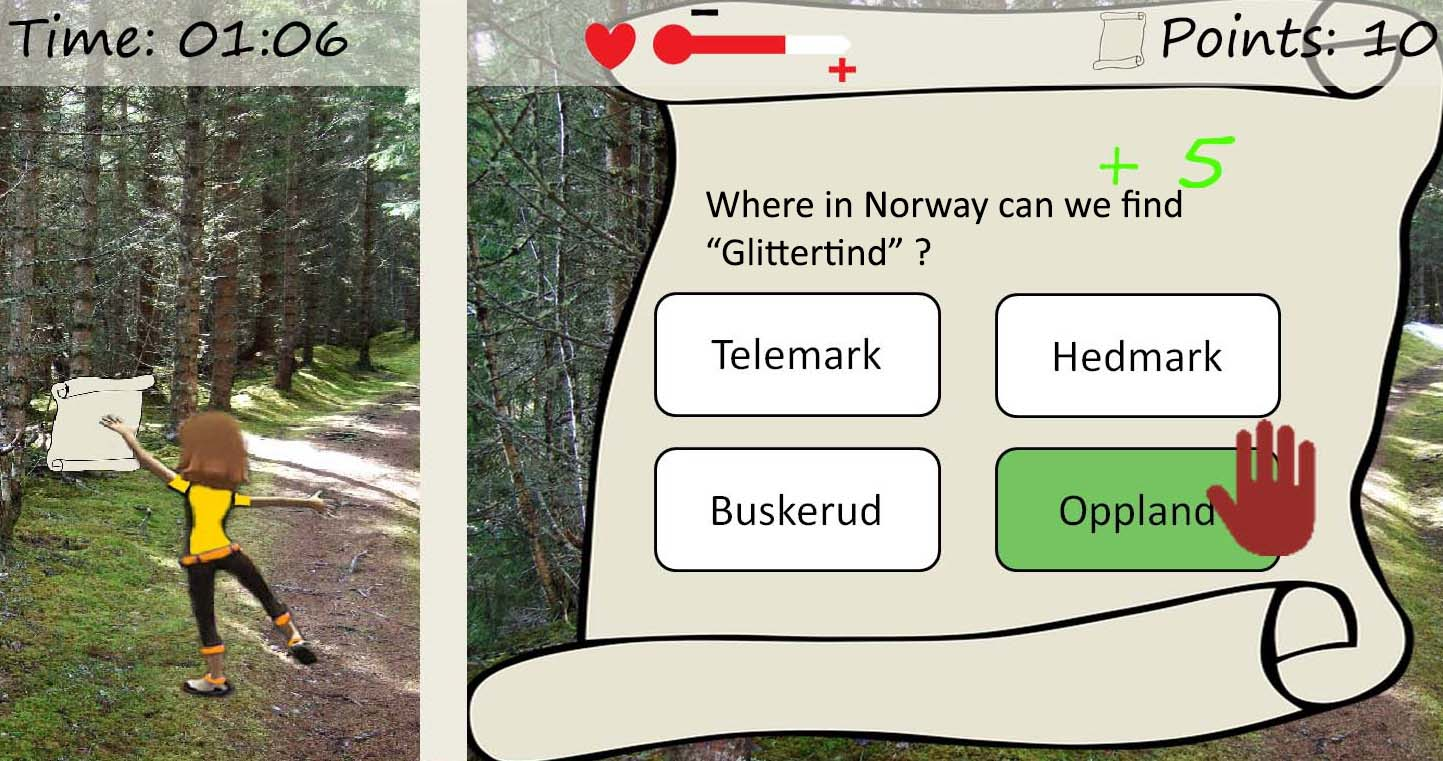
\includegraphics[scale=0.25]{quiznyengelsk.jpg}
\caption[Nature trail - quiz]{The quiz in the "Nature Trail" game will be shown as a piece of paper "hanging" on different spots in the forest. Questions will pop up and fill the screen. Here, the player is asked about where to find the Norwegian mountain "Glittertind".}
\label{fig:quiz}
\end{figure} 

Along the way in the nature trail there will be various, natural obstacles that will force the player to move her body in certain ways to be avoided. The game is supposed to exercise the whole body. Therefore, the different obstacles are chosen such that movements required to avoid them will include all muscle groups [req. 1.1, 1.3]. Examples of these obstacles are a river or creek that the player has to cross, or logs or rocks lying on the path that the player has to step over. To cross a river or creek the player has to balance on logs or step on rocks. This requires movements as toe-to-heel stepping, and step touch or skaters. When meeting a log, the player is required to take a big step, or a lunge, to get past it. Rocks in the path are avoided by performing sideways steps, or step-touch. There will also be obstacles in head height, like branches, which require the player to go into deep squats to be avoided. The Kinect sensor will track the player's body, and increase or decrease the "health-bar" according to how well the player performs the required movements. If the player hits some of the obstacles, they will get a flash of red, indicating that the player failed to avoid them. This is shown in Figure \ref{fig:hindring} f). As a result, the red colour in the "health-bar" will decrease [req. 1.20].

Parts of the story are organised with the use of "branching", which is about having the possibility to choose between multiple paths [req. 1.8]. An example is choosing between walking the "regular" trail and rowing a boat over a lake. To cross the lake, and continue the nature trail, the player has to take a side step into the boat. To move forward, rowing movements are needed. There will be water lilies on the lake, which the player has to avoid. This is done by leaning the upper body over to the sides. This, and all the other described obstacles, are shown in Figure \ref{fig:hindring}. All the tasks the player has to do throughout the game will be described in the functional design, in Section \ref{sec:functionaldesign}. The reader is referred to Appendix B for detailed instructions on how to perform the various exercises.

\begin{figure} [H]
\centering
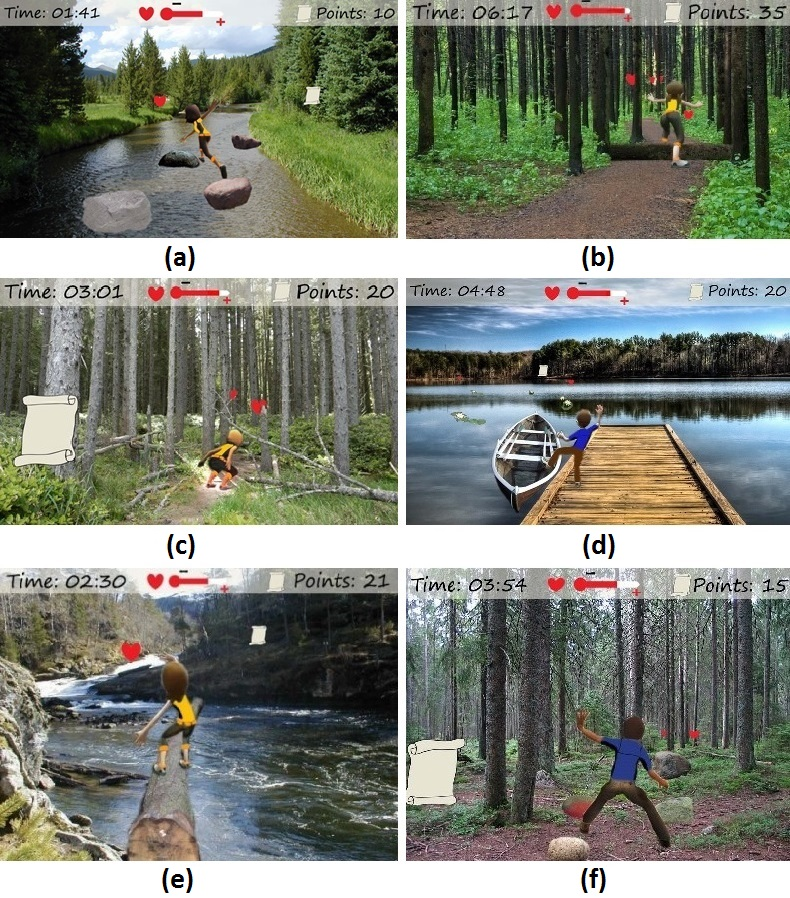
\includegraphics[scale=0.57]{hindringerEng.jpg}
\caption[Nature trail - obstacles]{This figure presents various obstacles to be found in the nature trail. a) jump from rock to rock to get over the river, b) walk over the log lying across the path, c) duck under the branch hanging over the path, d) get over the lake by rowing the boat, e) balance on the log to get over the river, f) walk pass the rocks lying on the path}
\label{fig:hindring}
\end{figure}

One of the requirements for this exergame is that the game has to show progress [req. 1.20]. In workshop 1, the informants told us that it is important to see that they are learning something, and that they feel that they get better. They also expressed it as important to get the possibility to choose difficult levels themselves. We have solved this by having a step in the menu where the player can choose the preferred difficulty for the game (see Figure \ref{fig:omgivelseNivaa}). To include the desire to experience progress and learning outcome, the game will be adjusted according to the player's current skills, where higher difficult levels will be accessible only when the player is "good enough". 

\begin{figure} [H]
\centering
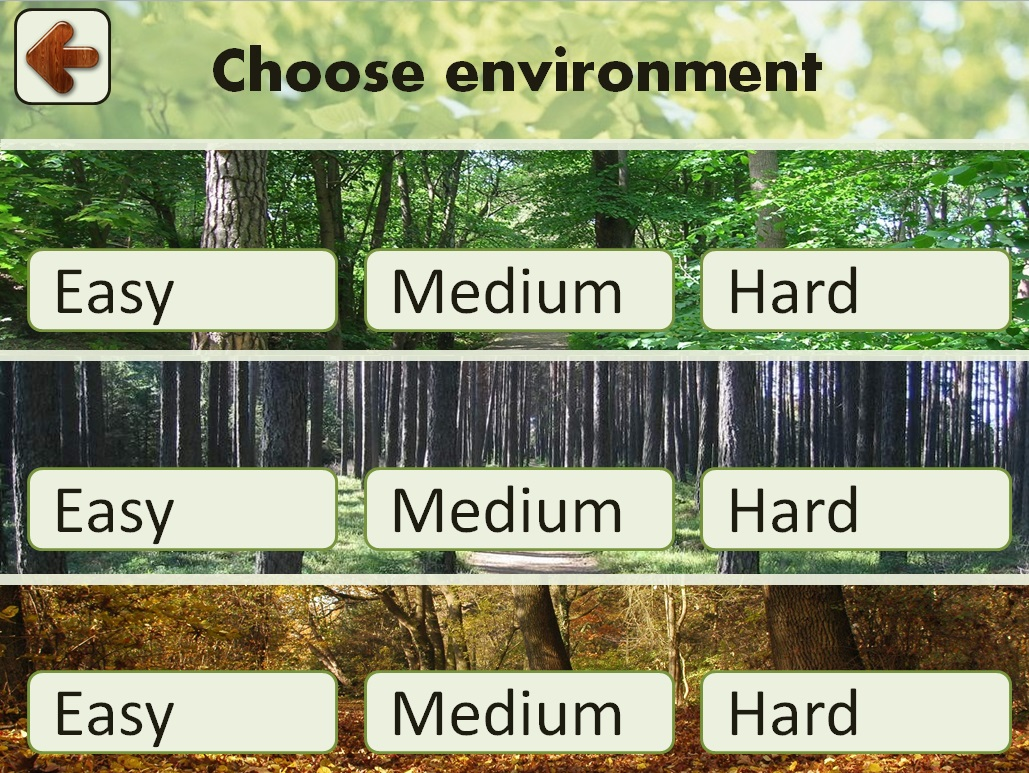
\includegraphics[scale=0.25]{chooseEnvironment.jpg}
\caption[Choice of environment and difficulty level]{The players will get the possibility to choose environment and difficulty level. The environments to choose from are pine wood, deciduous wood summer, and deciduous wood autumn; within each environment there are three difficulty levels.}
\label{fig:omgivelseNivaa}
\end{figure}

The "Nature Trail" game offers three different forest environments to walk in: a pine wood, and two deciduous woods, showing both summer and autumn. Each of the environments presents initially different difficulty levels, and within each environment, there are three difficulty levels: easy, medium, and hard [req. 1.8, 1.23]. First time playing, only the easy level will be available. The higher levels will be unlocked when the player has managed the easy level [req. 1.25]. A higher difficulty level will require more from the player, both mentally and physically. Obstacles will occur more frequently, which will require concentration, and the movements and exercises will be harder to perform, and therefore require control of the body. Within one environment, the obstacles from the easy level will follow to the next levels. This is done to include some familiar elements in the higher levels, in addition to new obstacles that will be added. To support variation between the environments, new and different obstacles will be used in each of the three environments.  

The required movements in the "Nature Trail" game are supposed to exercise the whole body. This involves endurance, balance, and exercise of several muscle groups. This game, with the quiz and movements combined, will be good for both cognitive skills and physical health.     

\subsection{The Four Single Games}
In addition to the "Nature Trail" game, "Out in the Nature" consists of four shorter games with focus on completing one single familiar activity or challenge. The activities we have chosen for this exergame are wood chopping, paddling down a river, swimming in a lake, and picking apples [req. 1.4, 1.6]. Within each game the player has the possibility to choose number of players and difficulty level [req. 1.8, 1.21, 1.23]. In multi-player mode, players can choose if they want to collaborate or compete against each other [req. 1.22]. When competing, the players will have the possibility to select difficulty level individually. This is to allow for players with different experience to play together, like a grandmother and her grandchild [req. 1.24]. Figure \ref{fig:velgSpill} shows how these single games will be presented in a menu. Below, we will describe one of these four games in more detail.

\begin{figure} [H]
\centering
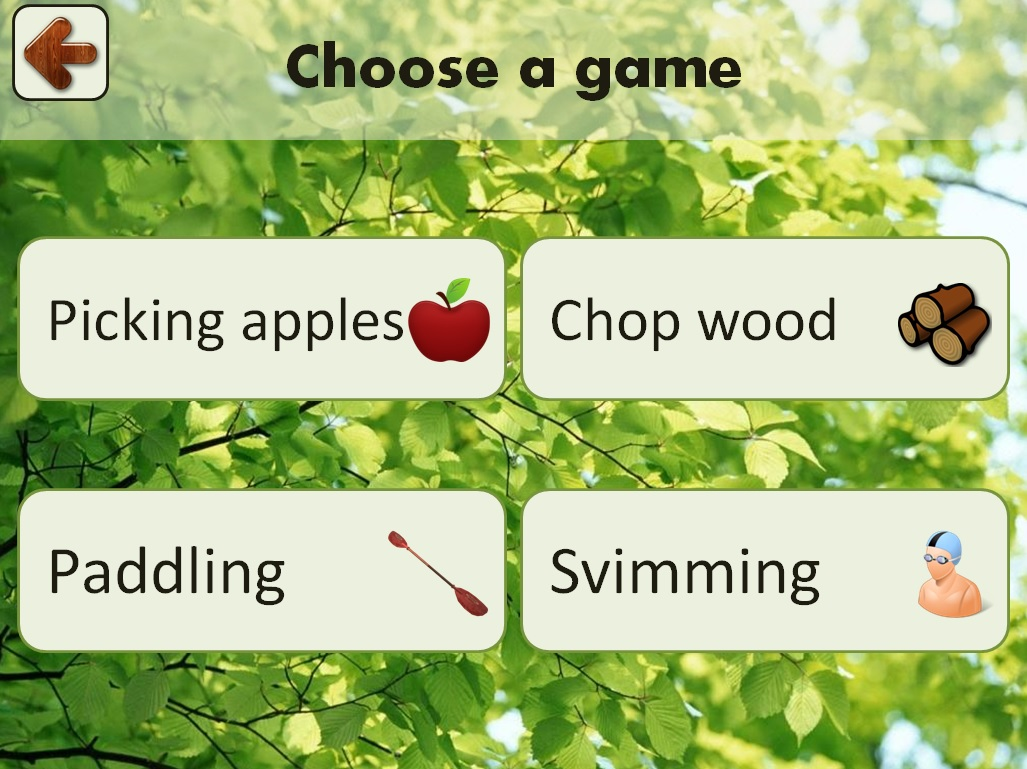
\includegraphics[scale=0.25]{chooseGame.jpg}
\caption[The four single games]{In addition to the "Nature Trail" game the players can choose between four single games: "Picking Apples", "Chopping Wood", "Paddling", and "Swimming".}
\label{fig:velgSpill}
\end{figure}

\subsubsection{Picking Apples}
"Picking Apples" is a game that requires squats and stretching exercises, which will strengthen balance and muscles in thighs and the gluteal area. The goal for this game is to pick as many red, ripe apples as possible in a given amount of time, and put them in baskets on the ground [req. 1.6]. This is shown in Figure \ref{fig:appleStretch} and \ref{fig:appleSquat}. The movements this game requires fit well with one of the chosen exercises from \emph{Øvelsesbanken} (see Figure \ref{pickingapples}). When apples first appear on the tree they will be green, indicating that they are not ready to be picked. If ripe apples are left hanging on the tree for too long, they will rot and fall to the ground. Rotten apples will have a brown colour. 

\begin{figure} [H]
\centering
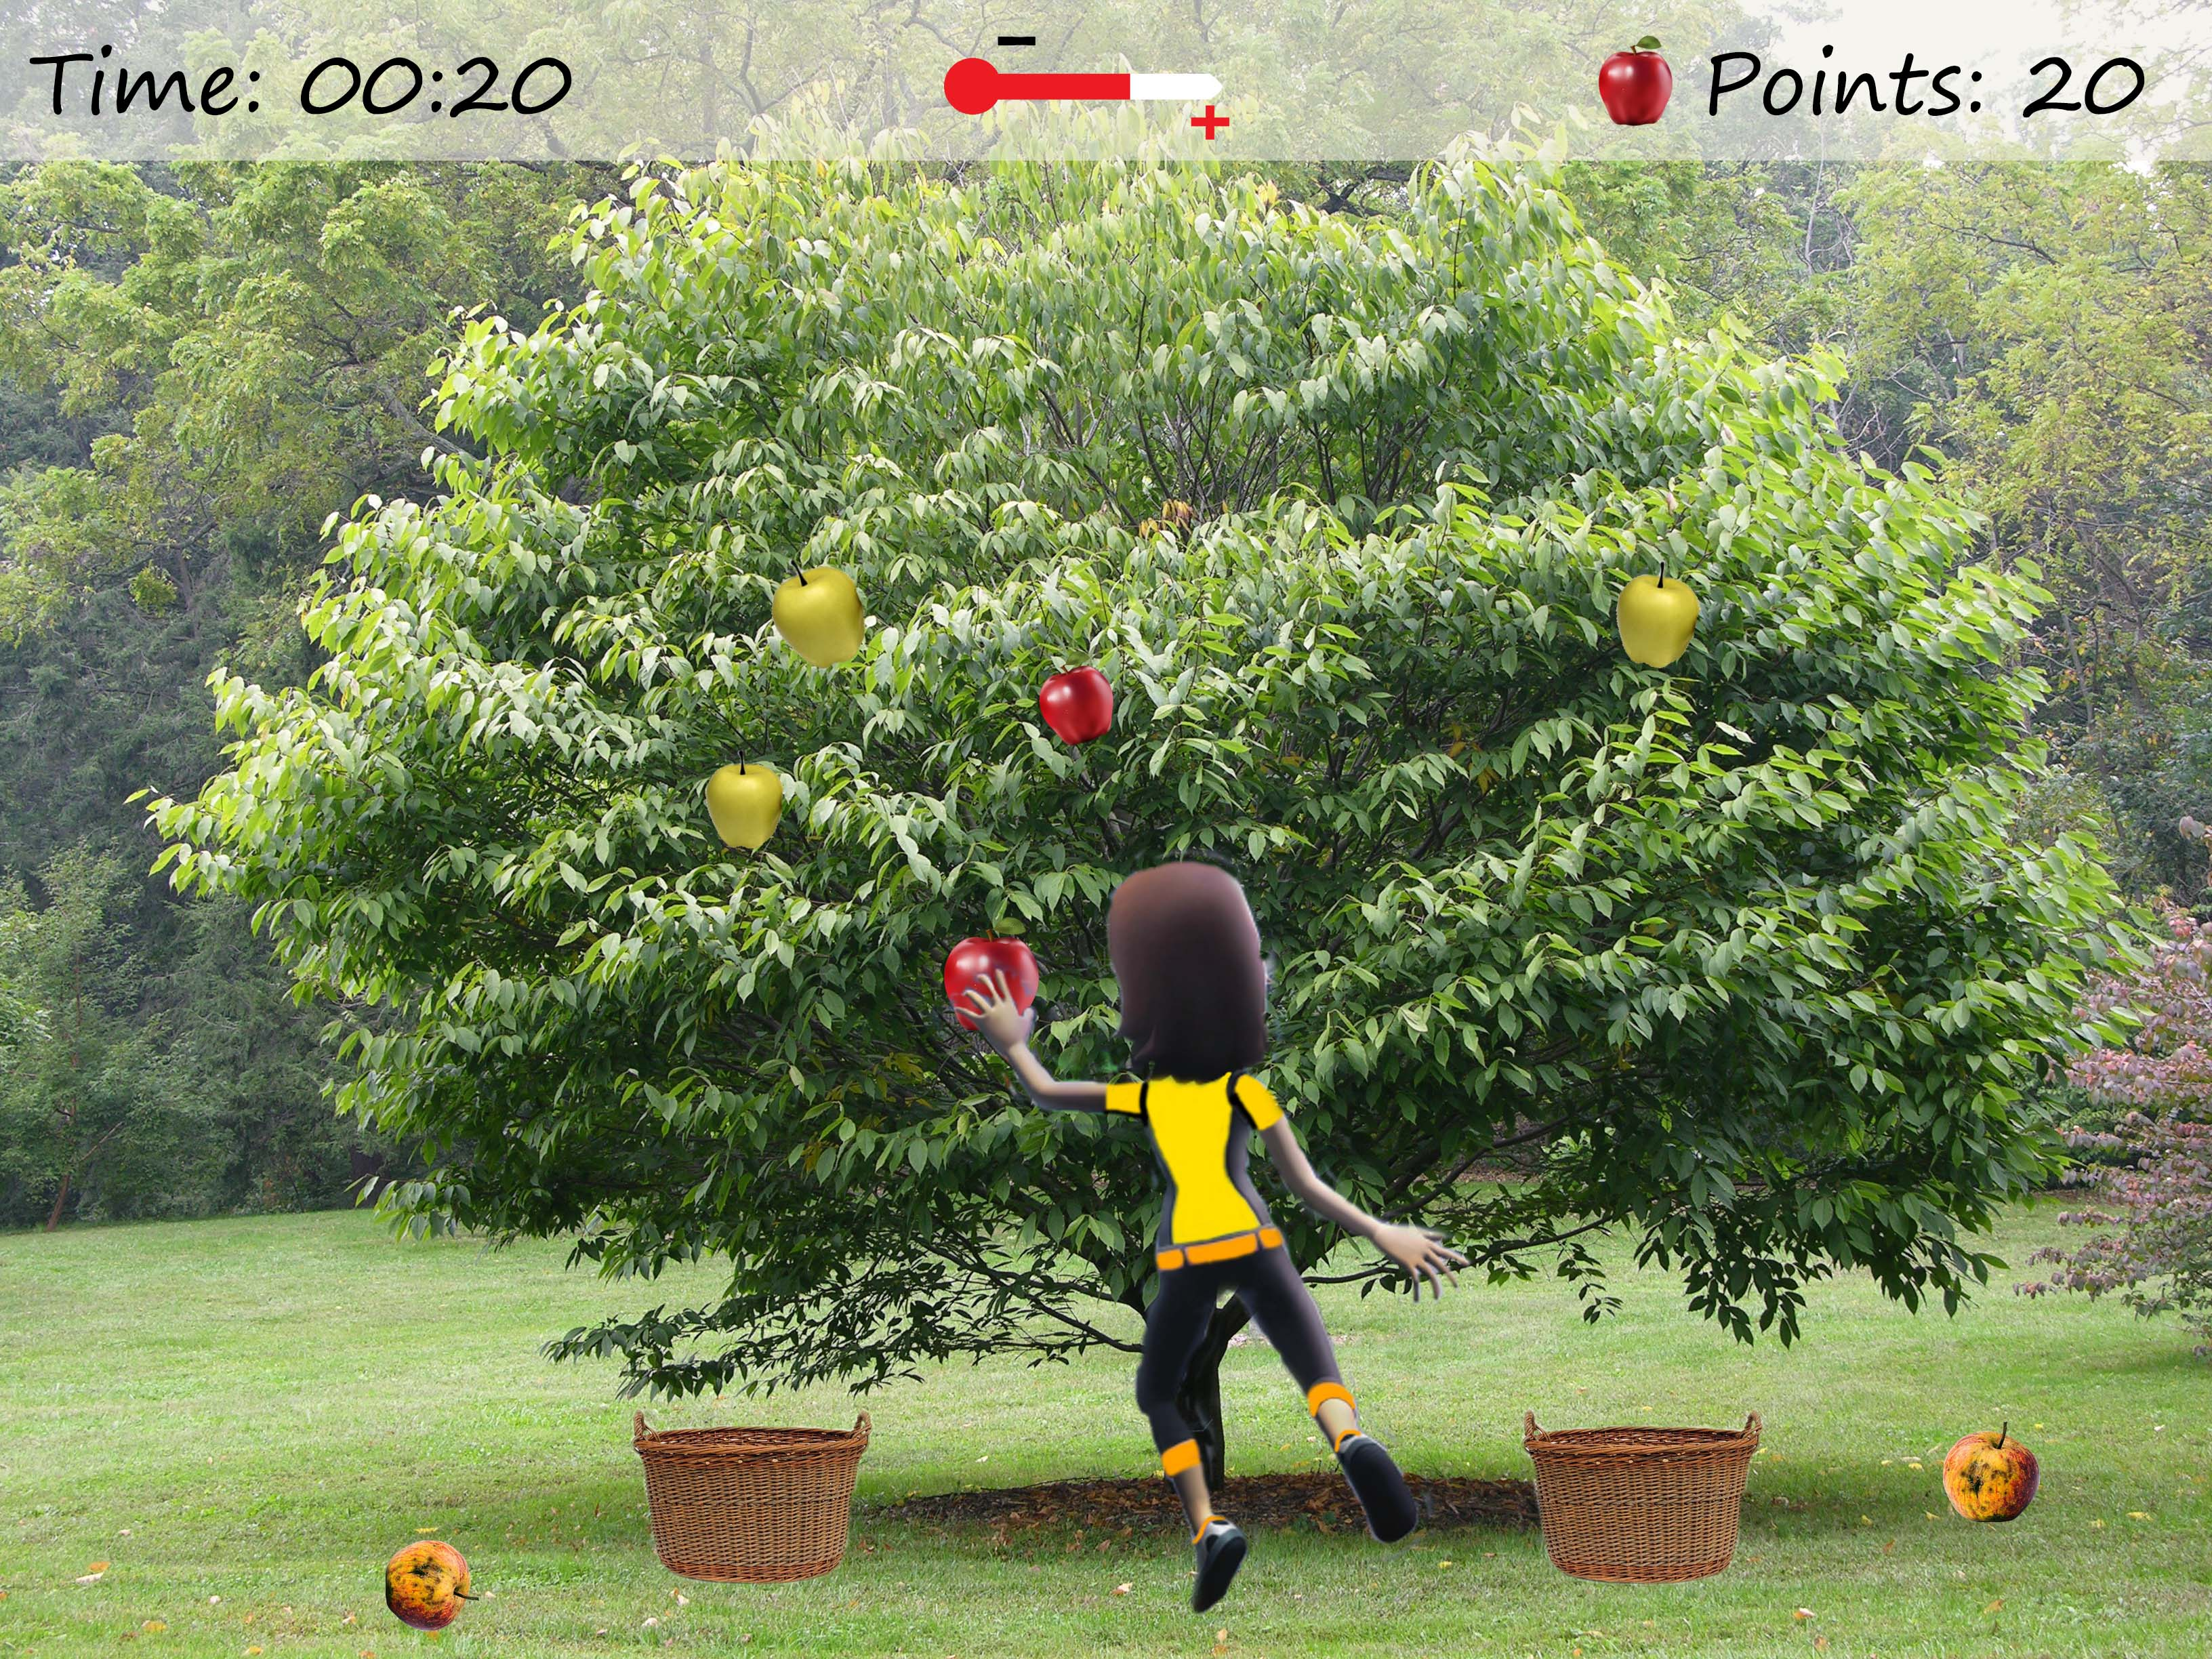
\includegraphics[scale=0.07]{gameappletreeEng.jpg}
\caption[Picking apples - stretching]{The player stretches up to pick a red, ripe apple. We observe that there are, in addition to red apples, three green apples on the tree, and two rotten on the ground.}
\label{fig:appleStretch}
\end{figure}

\begin{figure} [H]
\centering
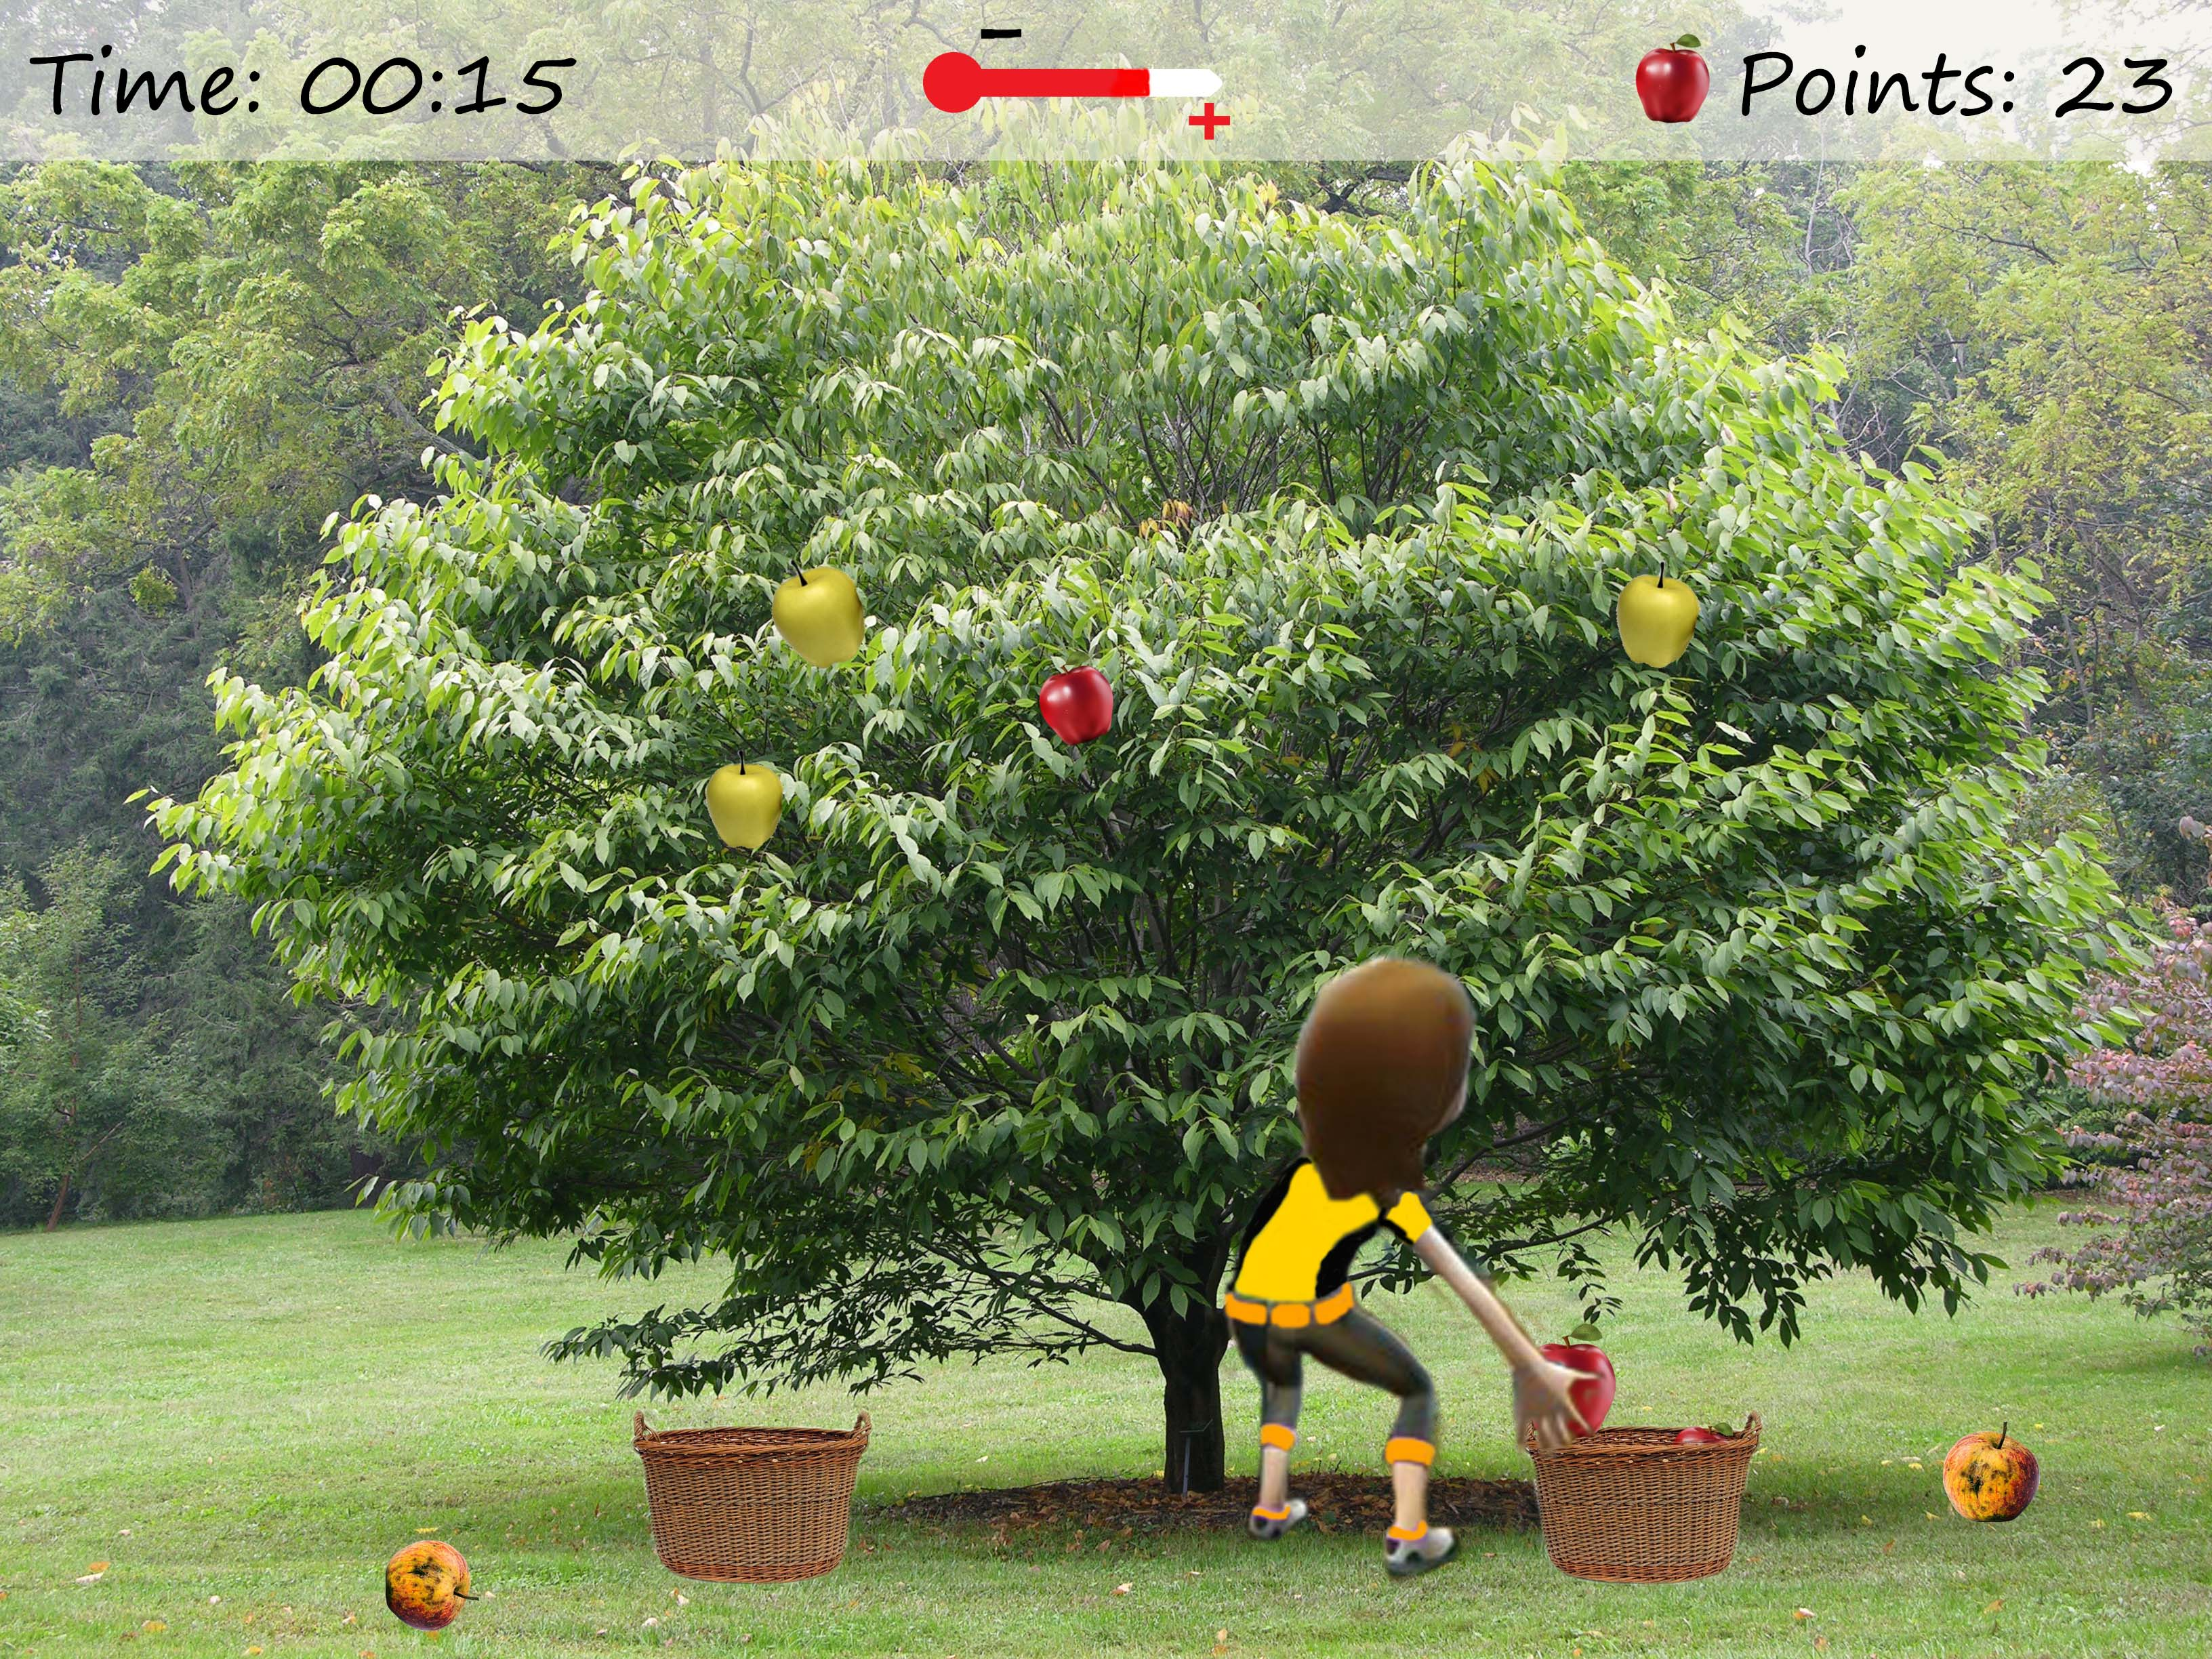
\includegraphics[scale=0.07]{squatppletreeEng.jpg}
\caption[Picking apples - squats]{The player has picked a red apple and is about to put it in the basket. The player uses deep squats to perform this action.}
\label{fig:appleSquat}
\end{figure}

Points will be given according to how many apples the player has picked (see Figure \ref{fig:appleOver}). 3 points will be given for each ripe apple that is picked and put in a basket. The player will lose points if green apples are picked, or if apples have been given the time to rot. Picking a green apple will result in -1 point, and if the apple gets rotten this will result in -2 points. If the player does not perform squats when putting apples in a basket, there is a great possibility that the apple will miss the basket and fall to the ground. This will give the same loss of points as a rotten apple, i.e. -2 points.       

\begin{figure} [H]
\centering
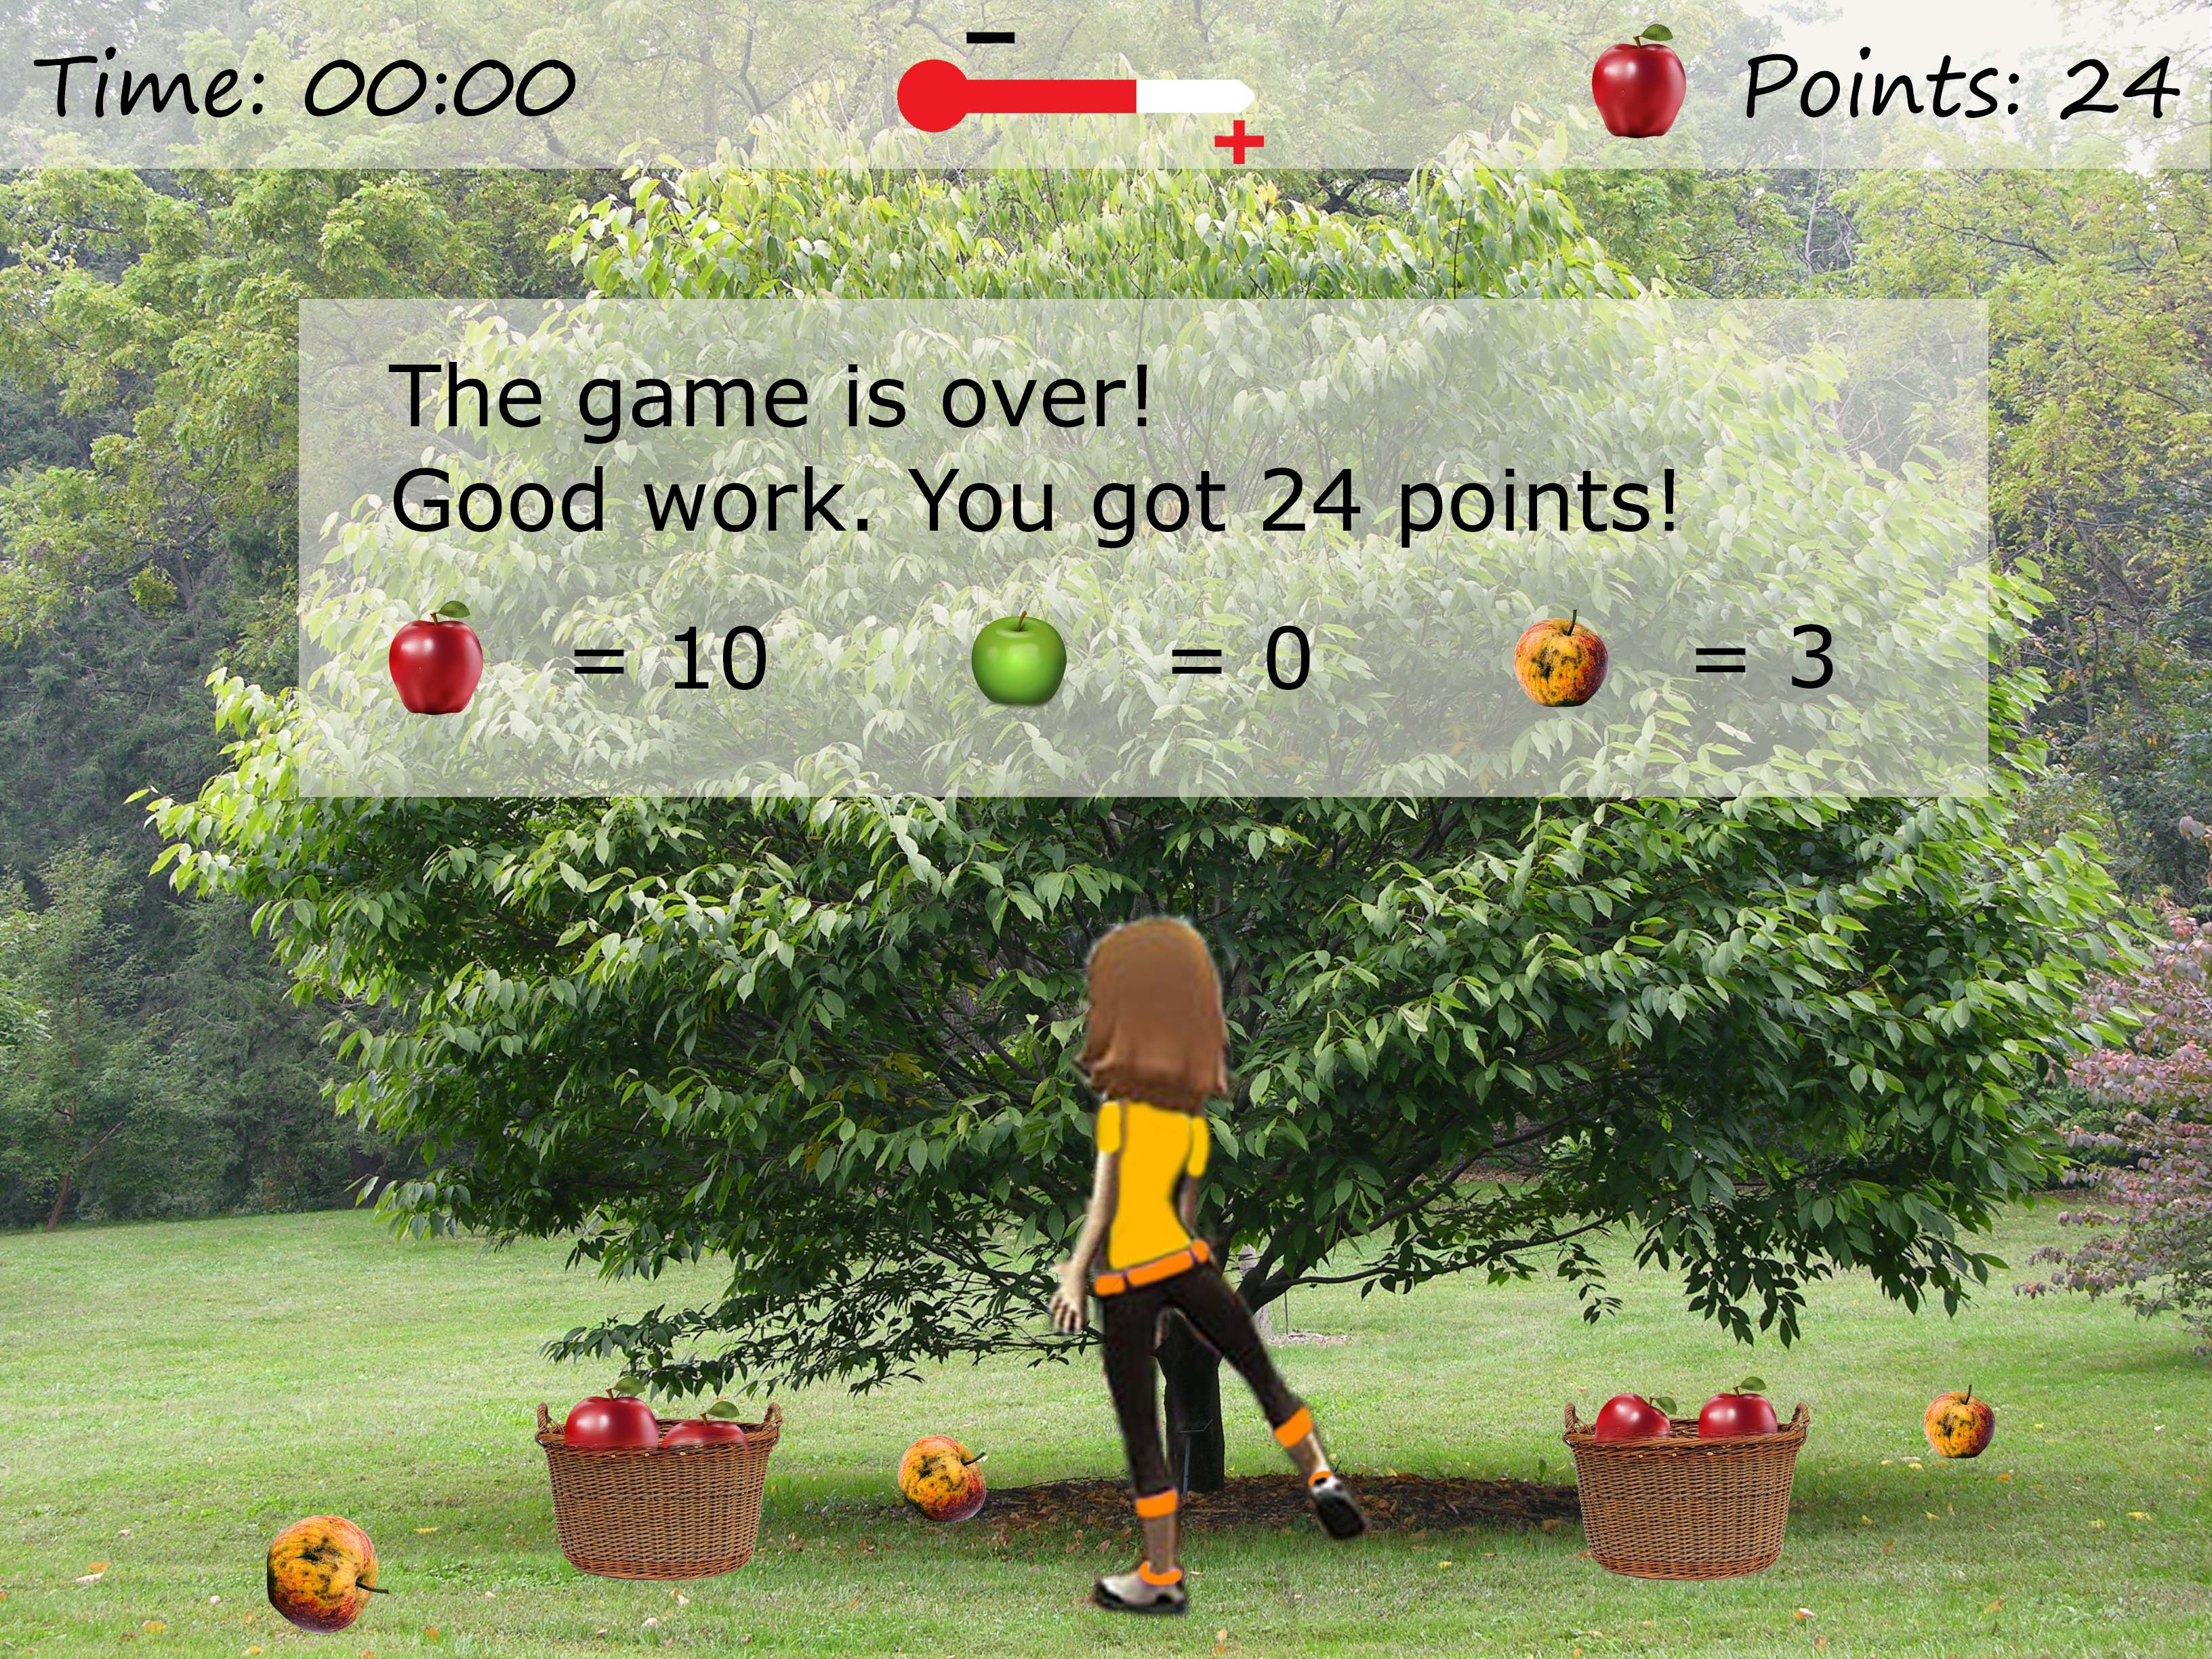
\includegraphics[scale=0.07]{appletreeendEng.jpg}
\caption[Picking apples - points]{This figure presents a final scene in the "Picking Apples" game. A text, together with the number of apples picked, is shown.}
\label{fig:appleOver}
\end{figure}

Apples will appear on the tree and grow in a certain tempo according to the chosen difficult level. A higher difficulty level will result in more apples on the tree at the same time, and a faster ripening rate. An additional challenge in a higher difficulty level is to have requirements to the two baskets, such as where the newly picked apple should be put. This is to train cognitive skills and to include more variation in movements and exercises [req. 1.24]. As mentioned, this game allows for multi-player mode where the players can collaborate on picking apples, or compete on who can pick the most apples (see Figure \ref{fig:appleMultiplayer}) [req. 1.22]. 

\begin{figure} [H]
\centering
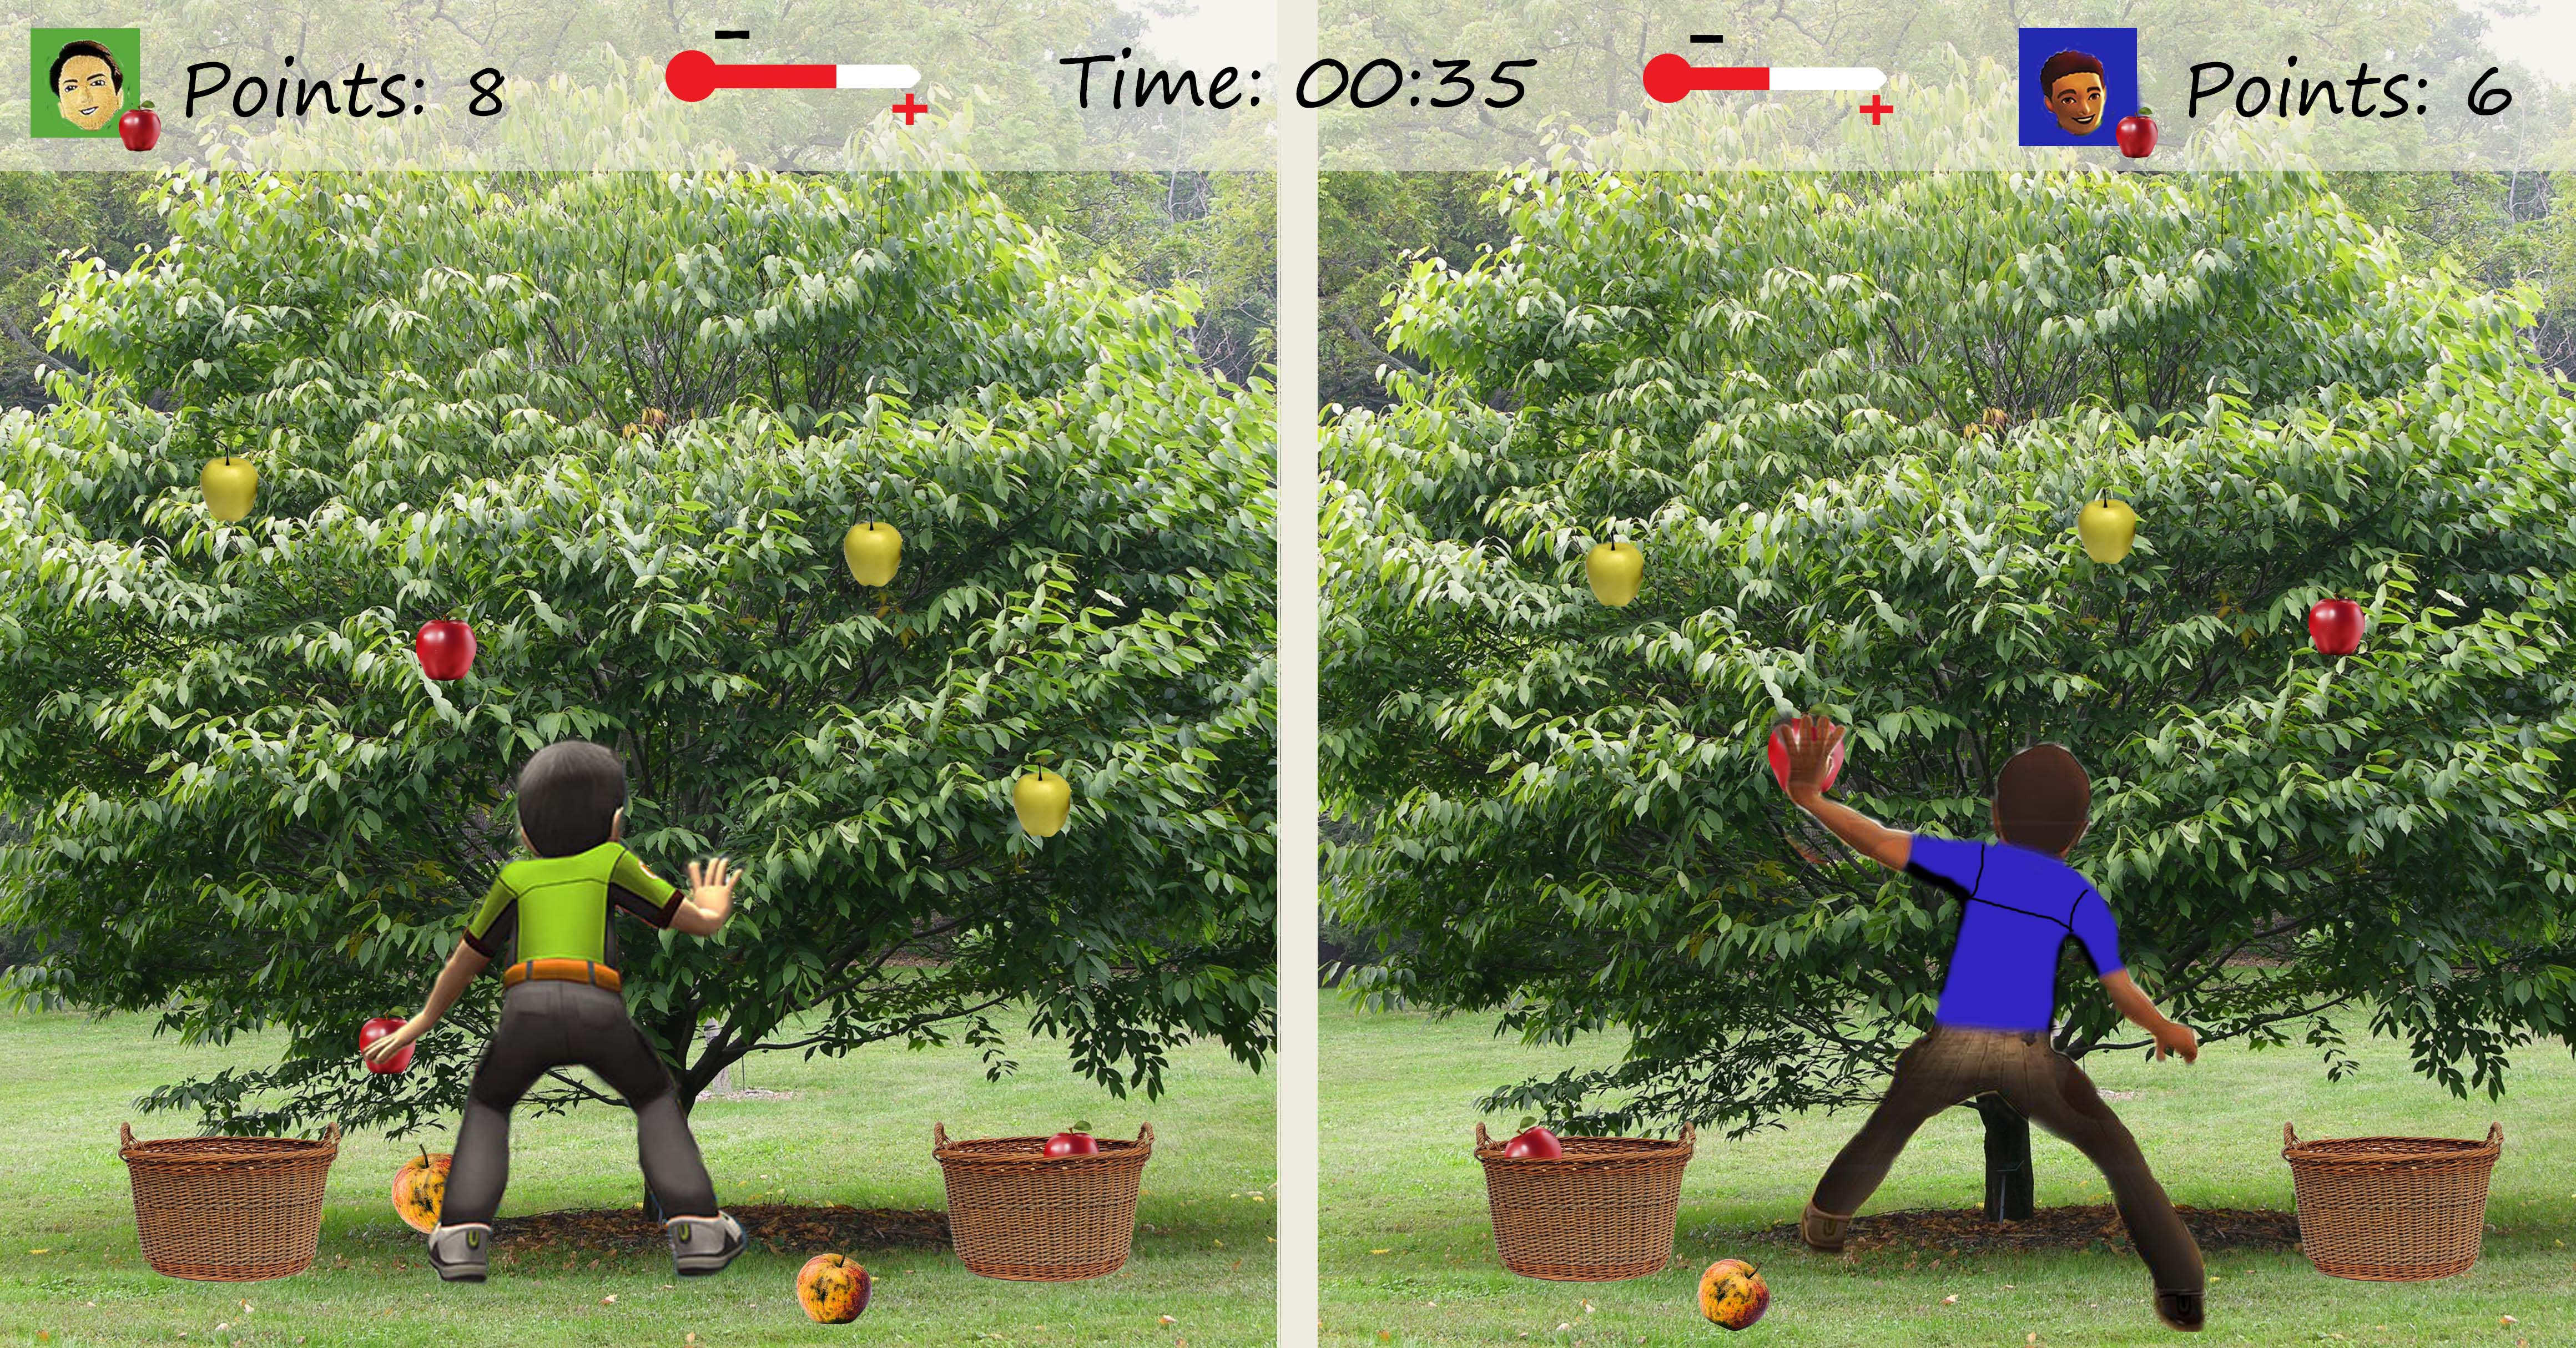
\includegraphics[scale=0.07]{gameapple2playerEngelsk.jpg}
\caption[Picking apples - multi-player]{In this figure we observe two players playing together in competitive mode.}
\label{fig:appleMultiplayer}
\end{figure}

\section{Functional Design}
\label{sec:functionaldesign}

The functional design for this game will be described according to system requirements presented in Section \ref{sec:req}, and to video game theory discussed in Chapter \ref{chap:vg}. The functional design will provide a more concrete representation of the exergame, than what have been presented earlier in this chapter. To get the overall picture of the game, Section \ref{sec:outinthenature} should be read before reading this section. Here, all the elements the game should contain will be presented shortly. Functional design will vary according to the chosen difficulty level; however, in this thesis we will only focus on presenting functional design for one difficulty level for each game. This will, as mentioned, be described according to video game theory, and more specifically to the game's story and aesthetics.  

\subsection{Nature Trail}

\subsubsection{The Fictional World} 

\begin{table} [H]
\centering
\begin{tabular}{|p{3,2cm}|p{7,8cm}|}
\hline
\emph{Location/setting} & In the pine forest  \\ \hline
\emph{Structural objects} & Trees, the trail, heaven, rocks, log, lake, puddle, creek, river.  \\ \hline
\emph{Interactive objects} & The player character, row boat with oars, rocks lying in the middle of the trail, rocks in the river, logs over a creek, red hearts in the field, branches, question sheets, log lying across the trail. \\ \hline
\emph{Scripting objects} & Quiz points: Shown as an icon similar to a sheet of paper, with the text "points" after it. Increments with 5 points as the player answer the right question.\\ \hline
	     & "Health-bar": Increases as the player performs right movements. Decreases as the player does not manage the right movements. Increases when the player gathers hearts. Increases based on time spend in game world compared to previous sessions. 
	      \\ \hline
	       & Time: Increases as a normal clock \\ \hline
\emph{Characters} & An avatar (from how Kinect defines a character) seen in third-person perspective, described by its name. \\ \hline
    \end{tabular}
    \caption[Various objects in the "Nature Trail"]{Different types of objects}
    \label{tab:objects1}
\end{table}  

\subsubsection{Mechanics} 

The game is a progression game, where a story should be completed. Each level will be completed by doing a certain sequence of quests or solving puzzles. The player has to finish different quests within a level to proceed to the next level, and the levels build on each other. It is common to have a climax at the end of each chapter in these type of games \cite{understandingvg}. However, this is not included here, as this will interfere with the natural environment and the gaming experience for this type of users. In Table \ref{tab:quests1} we will present different quests in the "Nature Trail" game. Branching are shown in Figure \ref{fig:flowchart}.
  
\begin{table}
\begin{tabular}{|>{\raggedright}p{7,5cm}|p{3,5cm}|}
\hline
\textbf{Quest} & \textbf{Exercise required}  \\ \hline
Walk on the trail to get forward in the forest & Walking, lift legs high \\ \hline
Gather hearts and "get better health" &  Stretching \\ \hline
Walk past rocks lying in the middle of the trail & Side steps or step touch  \\ \hline
Duck under branches hanging over the trail & Squats
\\ \hline
Balance over the log to get to the other side of the creek & Toe-to-heel stepping with arms out \\ \hline
Walk over the log lying across the trail & Lunges \\ \hline
Jump from rock to rock to get over the creek & Step touch or skaters \\ \hline
Row boat over to the other side of the lake & Rowing \\ \hline
Row past the water lilies & Lean upper body from side to side \\ \hline
Find and get question sheets  & Stretching \\ \hline
Answer one of the four alternatives & Use knowledge and cognitive skills \\ \hline
Solve puzzle & Use knowledge and cognitive skills \\ \hline
\end{tabular}
\caption[Quests in the "Nature trail" game]{Quests}
\label{tab:quests1}
\end{table}
 \newpage
 
\emph{Branching}

The two flow charts shown in Figure \ref{fig:flowchart} show how the story can be organised with "branching". In Figure \ref{fig:flowchart} (a), the player can choose to walk trail 1 without obstacles and hearts. This trail can be done just by walking. In trail 2, on the other hand, there are obstacles that need to be avoided, and hearts to gather. This trail will take some more time, but at the same time, exercise more of the body, which might result in a better score. In Figure \ref{fig:flowchart} (b) the player can choose to walk the trail without obstacles and hearts, or choose to row a boat over to the other side of a lake. The latter is shorter, but has water lilies that need to be avoided, and hearts to be gathered. There is a great chance for a total better score, by choosing to row the boat, as more of the body gets exercised. After finishing the chosen trail, the player will end up on the same trail again.

\begin{figure} [H]
\centering
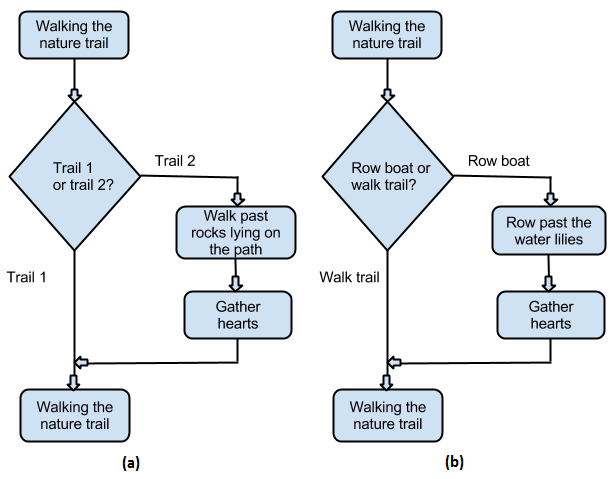
\includegraphics[scale=0.77]{flowchart}
\caption[Flow chart of branching]{Flow charts of two ways of "branching" in the game. (a) The player can choose between two different trails (b) The player can choose between walking the trail or rowing a boat over to the other side of a lake.}
\label{fig:flowchart}
\end{figure} 

\subsubsection{Rules} 
 
\begin{table}
\centering
\begin{tabular}{|p{2,8cm}|p{8,2cm}|}
\hline
\emph{Interplay rules} & \textbf{1. The player character:} Will move to the movements received as player input. \\ \cline{2-2}
&  \textbf{2. Red hearts:} When touched by the avatar it disappears. \\ \cline{2-2}
& \textbf{3. Rocks lying in the middle of the trail:} If hit, the  rocks will flash red.  \\ \cline{2-2}
&  \textbf{4. Branch:} If hit, it will flash red \\ \cline{2-2}
& \textbf{5. Log over creek:} If the avatar falls off, the log will flash red. \\ \cline{2-2}
& \textbf{6. Log across the trail:} If hit, the log will flash red.  \\ \cline{2-2}
& \textbf{7. Rocks in the river:} If the avatar falls of a rock, the rock will flash red.  \\ \cline{2-2}
& \textbf{8. Rowboat with oars:} Will move forward as the player uses her arms with the oars. \\ \cline{2-2}
& \textbf{9. Water lilies:} If hit, the water lily will flash red \\ \cline{2-2}
&  \textbf{10. Question sheets:} When touched by the avatar  it  disappears from the game environment and fills the screen with  a  question or puzzle. \\ \hline
\emph{Evaluation rules} & \textbf{if 1}: Player gets forward in the game, and the health-bar fills with red colour. \\ \cline{2-2}
& \textbf{if 2:} The health-bar fills with red colour.  \\ \cline{2-2}
& \textbf{if 3:} Player gets slowed down, and red colour in the health-bar reduces.   \\ \cline{2-2}
& \textbf{if 4:} Player gets slowed down, and red colour in the health-bar reduces.  \\ \cline{2-2}
& \textbf{if 5:} Player gets slowed down, and red colour in the health-bar reduces   \\ \cline{2-2}
& \textbf{if 6:} Player gets slowed down, and red colour in the health-bar reduces   \\ \hline
\end{tabular}
\caption[Rules in the "Nature Trail" game]{Rules}
\label{tab:rules1}
\end{table} 

\begin{table} [H]
\centering
\begin{tabular}{|p{2,8cm}|p{8,2cm}|}
\hline
\emph{Evaluation rules} & \textbf{if 7:} Player gets slowed down, and red colour in the health-bar reduces   \\ \cline{2-2}
& \textbf{if 8:} Player gets forward in the game, and the health-bar fills with red colour.   \\ \cline{2-2}
& \textbf{if 9:} Player gets slowed down, and red colour in the health-bar reduces   \\ \cline{2-2}
& \textbf{if 10:} If player answers right she gets +5 points. If player answers wrong she gets 0 points.  \\ \hline
\end{tabular}
\caption[Rules in the "Nature Trail" game]{Rules continues}
\label{tab:rules11}
\end{table}  

\subsubsection{Geography and Representation}

\begin{table} [H]
\centering
\begin{tabular}{|p{2,7cm}|p{8,3cm}|}
\hline
\emph{Music} & Calm, classical music that changes to the speed of the game and to certain happenings. \\ \hline
\emph{Vocalization} & The avatar will not have its own voice. \\ \hline
\emph{Sound effects} &  When hearts are gathered there is a cheerful "pling" sound.  \\ \cline{2-2}
&  When taking the question sheet there is a "click" sound.\\ \cline{2-2}
& When the avatar is walking there is the sound of steps on the ground. Different sounds for \\ & different surface, i.e. walking on the rocks, soil or logs.\\ \cline{2-2}
& The sound of shoved water when rowing. \\ \hline
\emph{Ambient effects} & Birdsong. \\ \cline{2-2}
& Wind. \\ \cline{2-2}
& Water flowing in the river. \\ \cline{2-2}
& Waves from the lake.\\ \hline
\emph{Feedback} & Calm lady voice. \\ \hline
\end{tabular}
\caption[Different types of sound]{Different types of sound}
\label{tab:sound1}
\end{table}  

\begin{table} [H]
\centering
\begin{tabular}{|p{2,5cm}|p{8,5cm}|}
\hline
\emph {Perspective} & Third-person. \\ \hline
\emph{Dimension} &  3-dimensional and isometric. \\ \hline
\emph{Exploration} & Desired pace. \\ \hline
\emph{Saving} & The game will be able to save current state, progress and results. \\ \hline
\emph{Graphical representation} & The environment will be presented as close to photorealism as possible.  However, there will be some unrealistic elements present in the game environment, i.e. hearts  \\ \hline
\end{tabular}
\caption[Graphical game characteristics]{Graphical game characteristics}
\label{tab:graphical1}
\end{table}  

\subsubsection{Number of Players}
The game supports two simultaneous players. The players can either compete or collaborate.

\subsection{Picking Apples}

\subsubsection{The Fictional World} 

\begin{table} [H]
\centering
\begin{tabular}{|p{3,2cm}|p{7,8cm}|}
\hline
\emph{Location/setting} & The player stands on a lawn with an apple tree in front of her. \\ \hline
\emph{Structural objects} & Tree, grass, heaven.  \\ \hline
\emph{Interactive objects} & The player character, apples on the tree, two baskets, one on each side of the player. \\ \hline
\emph{Scripting objects} &  Points: Shown as an apple icon with the text "points" after it. Increments with 3 points as ripe apples are picked and decrements with -1 point if an unripe apple is picked, and -2 points if an apple gets rotten \\ \cline{2-2}
& "Health-bar": Increases as player performs right  movements. Decreases as player does not manage the right  movements.  \\ \cline{2-2}
& Time: Decreases from 2 minutes \\ \hline
\emph{Characters} & An avatar (from how Kinect defines a character) seen in third-person perspective, described by its name. \\ \hline
\end{tabular}
\caption[Various objects in the "Picking Apples" game]{Different type of objects}
\label{tab:objects2}
\end{table}  
 
\subsubsection{Mechanics} 
This is a progression game where different level of the game gets finished by solving the apple-picking task. The player has to finish different levels to proceed to the next level. The levels build on each other and the difficulty level gets higher as the player proceeds through the game.

\emph{Quests:} 

\begin{table}
\begin{tabular}{|>{\raggedright}p{7,5cm}|p{3,5cm}|}
\hline
\textbf{Quests} & \textbf{Exercise required}  \\ \hline
Pick apples when they get red and ripe & Stretching  \\ \hline
Put ripe apples in baskets &  Squats with downward arm movement \\ \hline
\end{tabular}
\caption[Quests in the "Apple Picking" game]{Quests}
\label{tab:quests2}
\end{table}

\subsubsection{Rules} 

\begin{table} [H]
\centering
\begin{tabular}{|p{2,8cm}|p{8,2cm}|}
\hline
\emph{Interplay rules} & \textbf{1. The player character:} Will move to the movements received as player input. \\ \cline{2-2}
 &  \textbf{2. Apples on the tree:} Will appear on the tree with a green colour showing they are not yet ripe. After a while they will start to get red, and if the apples does not get picked while they are red, they will become brown and fall to the grown. \\ \cline{2-2}
& \textbf{3. Baskets:} The baskets will get filled with apples. \\ \hline
\emph{Evaluation rules} & \textbf{if 1:} Player proceeds through the game, and the health-bar fills with red colour.\\ \cline{2-2}
 & \textbf{if 2:} If the player picks a ripe apple she gets +3 points. If an apple becomes rotten the player gets -2 points. If the player picks an unripe apple she gets -1 point. \\ \cline{2-2}
& \textbf{if 3:} If the player puts ripe apple in the basket she keeps the 3 points. If the player miss the basket, she loses 2 points.  \\ \hline
\end{tabular}
\caption[Rules for the "Apple Picking" game]{Rules}
\label{tab:rules2}
\end{table}  

\subsubsection{Geography and Representation}

\begin{table} [H]
\centering
\begin{tabular}{|p{2,7cm}|p{8,3cm}|}
\hline
{Music} & Calm, classical music that changes to the speed of the game and to certain happenings. \\ \hline
\emph{Vocalization} & The character will not have its own voice. \\ \hline
\emph{Sound effects} & Apples making a "pling" sound when getting picked.  \\ \cline{2-2}
&  Apples hitting the ground when falling from the tree. \\ \hline
\emph{Ambient effects} & Birdsong. \\ \cline{2-2}
& Wind. \\ \hline
\emph{Feedback} & Calm lady voice. \\ \hline
\end{tabular}
\caption[Different types of sounds in the "Apple Picking" game]{Different types of sound}
\label{tab:sound2}
\end{table}  

\begin{table} [H]
\centering
\begin{tabular}{|p{2,5cm}|p{8,5cm}|}
\hline
\emph {Perspective} & Third-person \\ \hline
\emph{Dimension} &  3-dimensional and isometric \\ \hline
\emph{Exploration} &  A mix between forced and desired pace. The pace is forced because the apples appear at random times. At the same time the pace is desired because the player can choose when she wants to stretch to gather the apple. However, this can also mean that the player chooses to lose an apple. Ripening pace will depend on current difficulty level.\\ \hline
\emph{Saving} & The game will be able to save current state, progress and results. \\ \hline
\emph{Graphical representation} & The environment will be presented as close to photorealism as possible.  \\ \hline
\end{tabular}
\caption[Graphical game characteristics in the "Apple Picking" game]{Graphical game characteristics}
\label{tab:graphical2}
\end{table}  

\subsubsection{Number of Players} 
The game supports two simultaneous players. The players can either compete or collaborate. 


\section{The Menu}
\label{sec:menu}

One of the main challenges we observed during workshop 1 was related to handling the menus in the different games. The general perception from workshop 1 was that the menus were complex, difficult to follow, demanding to navigate through, and too sensitive. This was also our own experience from playing. Therefore, we have made a prototype of a menu, which will be presented in this section.

The design of our menu proposal is based upon the interface requirements, listed in Table \ref{tab:nfunc1} and \ref{tab:nfunc2}. Simple design, distinct elements, and easy to read information are emphasised to make it user-friendly for elderly that might suffer from declined vision [req. 2.6, 2.14, 2.16]. It has also been a focus not to have too much information in each menu step. We have chosen to make a menu consisting of more steps to achieve the mentioned goal. By having a bit longer menu, we avoid filling few menu steps with lots of information and choices [req. 2.12].    

The menu starts with the choice of how the player wants to play [req. 1.8]. The player can choose between a walk in the forest, to exercise a preferred muscle group, or between the four single games. If the player wants to play according to training a specific muscle group, she will be given the choice of which muscle group to exercise. Independent of how the player chooses how to play, she will be given the opportunity to choose difficulty level and number of players for the game [req. 1.21, 1.23]. Figures \ref{menu1} and \ref{menu2} go through the menu, from start, through choosing muscle group, to ending up playing "Picking Apples". As seen from what we have presented this far, the menu includes a lot of choices. This is based on the informants' feedback in workshop 1, where they said that they wanted the possibility to make their own choices. They did not want the game to control them.   

\begin{figure} [H]
\centering
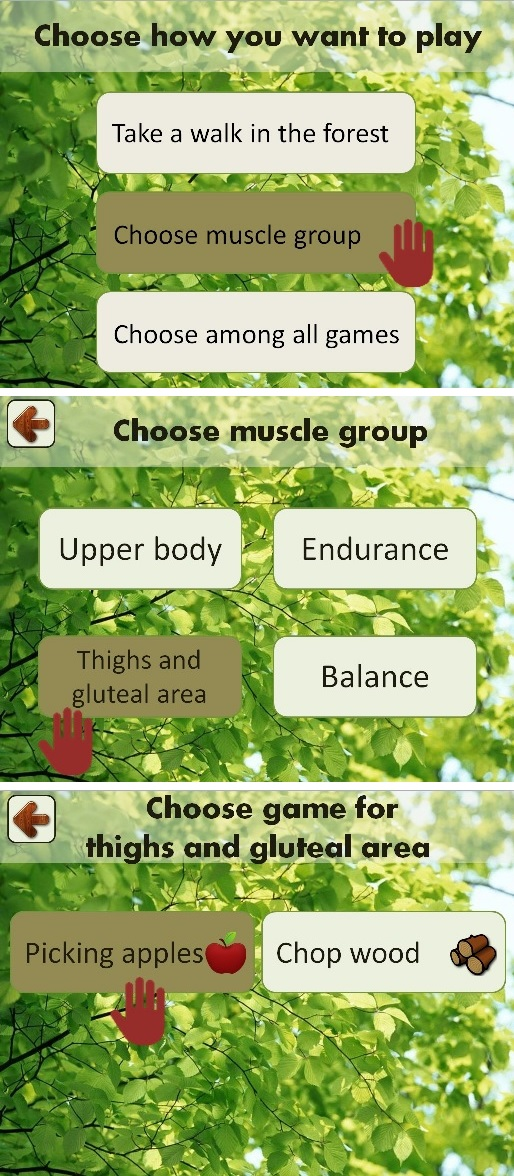
\includegraphics[scale=0.45]{menuEnglishStep1.jpg}
\caption[Menu review -  part one]{This figure shows the menu step by step, from the beginning to playing a single game, here "Picking Apples". The selection of single games is a result of the chosen muscle group.}
\label{menu1}
\end{figure}

\begin{figure} [H]
\centering
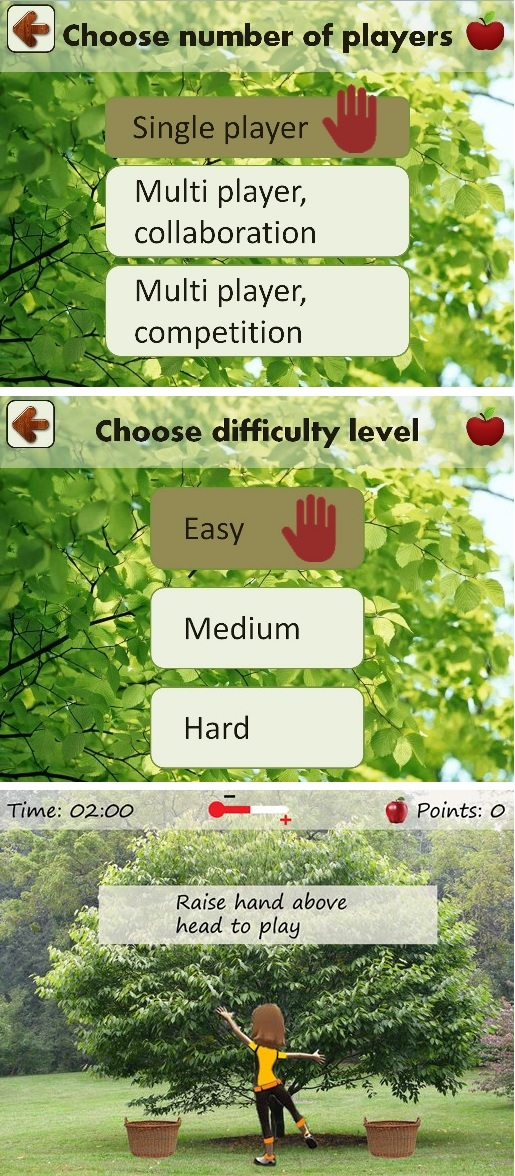
\includegraphics[scale=0.45]{menuEnglishStep2.jpg}
\caption[Menu review - part two]{This figure shows the menu step by step, from the beginning to playing a single game, here "Picking Apples". Single player game and the easy difficulty level are chosen.}
\label{menu2}
\end{figure}

In the menu, we have used a range of green colours, and a picture of green leaves as background, to create a theme related to forest and nature. Menu buttons are arranged as list elements or in a square, depending on what is most appropriate. This is decided by the number of elements in each step; for an odd number of elements, list view is used, while square arrangement is used for an even number of elements. The size of the elements is chosen with usability in mind; there should be room for a proper font size, and it should be easy to push the right button [req. 2.12]. The buttons have a light green, almost white, background colour, with a darker green outline. The text is written in black with an easy-to-read, sans serif font [req. 2.14]. The choice of background and text colour is to create maximum contrast [req. 2.15]. It is important to take the element's surroundings into account when choosing colours if you want to make the element stand out. With e.g. green vegetation as surroundings, white background colour, with black, dark green, or dark blue text should be chosen to create maximum contrast [req. 2.16]. 

\begin{figure} [H]
\centering
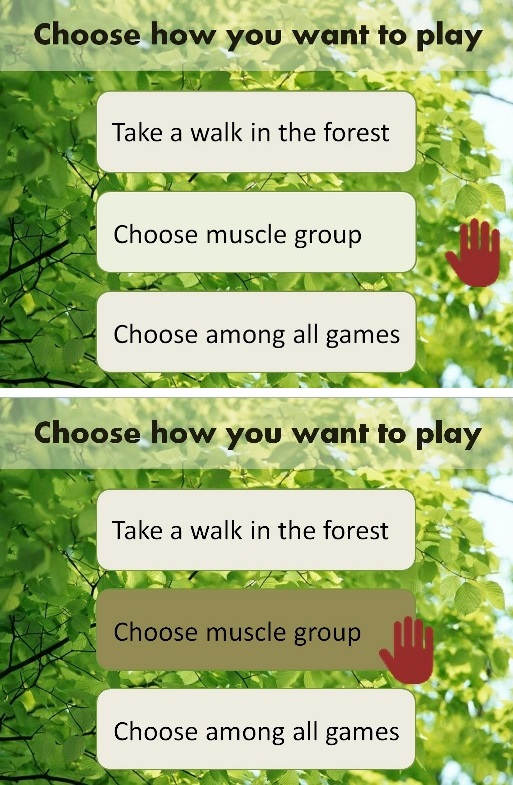
\includegraphics[scale=0.4]{menuAction.jpg}
\caption[Menu - Action and response]{In this figure an avatar hand is shown. The avatar hand will react according to the player's movements. We see that when the player move their arm over an element, it will change colour.}
\label{fig:avatarAction}
\end{figure} 

The title on each step is written in a bold, black, easy to read font, on a semi-transparent light-coloured background. The title is stating what choice to be made at the current step [req. 2.6]. We know from the previous chapters that it is important to have an interface with visible information, and that users always should be given feedback on their actions. Also, the informants in workshop 1 expressed that, it was general desire to see a more clear response on their actions. We have included this in our exergame by highlighting elements that are "in action" [req. 1.15], see Figure \ref{fig:avatarAction}. The player's hand movements are portrayed on the screen as an avatar hand. The avatar hand has been given a clear colour and a solid fill [req. 2.11]. This has been done to avoid having the same diffuse avatar hand as in "Your Shape Fitness Evolved 2012".  

\begin{figure} [H]
\centering
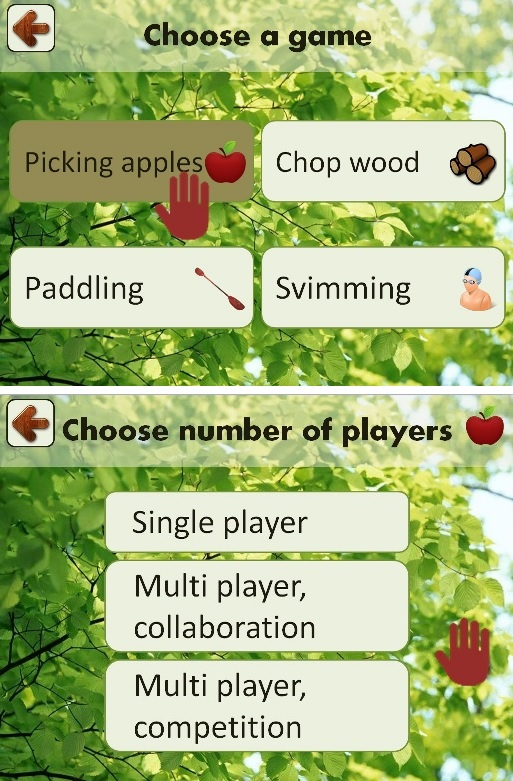
\includegraphics[scale=0.4]{menuIconApple.jpg}
\caption[Menu - use of icons]{In this figure we see that icons from the menu buttons will follow through the menu. Here we see that the apple icon will follow into the menu step where number of players are to be chosen.}
\label{fig:iconEple}
\end{figure} 

In the menu step where the player can choose between the four single games, we have used icons in addition to text on each button, see Figure \ref{fig:velgSpill}. The icons represent the challenges in each game, and they are meant to make it easier for the player to understand the game behind the button [req. 2.6]. When choosing a game, e.g. "Picking Apples", the icon will follow up in the right corner, to inform the player where she is headed, and to reduce memory load [req. 1.12]. This is shown in Figure \ref{fig:iconEple}.  

Up in the left corner there is a back button, which will make it possible for users to always regret their action [req. 1.30]. The back button is shaped and coloured similar to the other menu buttons to maintain consistency and intuitiveness [req. 2.6-7]. The choice of placement is based on the natural way to read and observe information, which is from top to bottom, from left to right. The navigation should therefore be on top [req. 2.12]. We avoided placing the back button in the bottom left corner to not mix it with the cancel/pause feature included in the Kinect software (holding your left hand straight 45 degrees from your body). The back button is marked with a wooden arrow, a familiar and intuitive icon related to navigation. The choice of using a wooden arrow is based on its relation to the forest theme. 
     
\section{A Video Game Series}
"Out in the Nature" is part of an exergame series called "Kinect Experiences". This series consist of four individual games with the same structure as the game we have already presented. This means, one compounded game and four single games. The difference between the exergames is the main themes. In addition to "Out in the Nature", the "Kinect Experience" series consist of the exergames "Farm Life", "On Vacation" and "In the Mountains". The five games within each exergame will consist of activities that are connected to the main theme of the exergame. Examples of single games can be gathering eggs, and stacking hay bales in "Farm Life", and a walk on the beach, or catching gold fish with a hoof in "On Vacation". The idea behind this video game series is to offer a wide range of games, activities and exercises that fits the various interests the user group have [req. 1.2, 1.4-5]. What this video game series would look like is shown in Figure \ref{fig:videogameseriesAlone}. 

\begin{figure} [H]
\centering
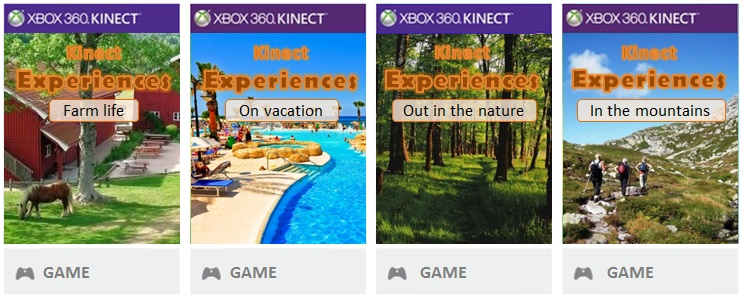
\includegraphics[scale=0.65]{videoGameSeriesAlone.jpg}
\caption[Presentation of our video game series]{A presentation of our video game series "Kinect Experiences" (modified from \cite{XboxNettside}).}
\label{fig:videogameseriesAlone}
\end{figure}

